% ================================================================
%  IEEE Transactions-style Research Paper
%  Enhanced FDI Attack Detection in EV Charging Networks via
%  NARX + Attention-BiLSTM with Adaptive Two-Stage IF-CUSUM
% ================================================================
\documentclass[journal]{IEEEtran}

\usepackage{amsmath, amssymb, amsfonts}
\usepackage{algorithm}
\usepackage{algorithmic}
\usepackage{graphicx}
\usepackage{textcomp}
\usepackage{xcolor}
\usepackage{booktabs}
\usepackage{multirow}
\usepackage{cite}
\usepackage{url}
\usepackage{tikz}
\usetikzlibrary{shapes.geometric, arrows, positioning, fit, calc}

\graphicspath{{results/}}

% ----------------------------------------------------------------
\begin{document}

\title{Stealthy Metering Integrity Attack Detection in Smart EV        
  Charging Infrastructure Using Attention-Based Bidirectional LSTM 
  with Adaptive Isolation Forest–CUSUM}

\author{Sudarshan~Sudhakar,~\IEEEmembership{Student~Member,~IEEE}
\thanks{Manuscript received April 2026.
S.~Sudhakar is with the Department of Information Security,
School of Computing, Vellore Institute of Technology,
Chennai 600127, India
(e-mail: sudarshan.sudhakar@ieee.org).}}

\maketitle

% ----------------------------------------------------------------
\begin{abstract}
False Data Injection~(FDI) attacks on Electric Vehicle~(EV)
charging infrastructure represent a critical class of cyberthreat
that simultaneously compromises billing integrity, grid scheduling
accuracy, and demand-response reliability.
Existing detection schemes rely either on simplistic statistical
thresholds that fail under low-amplitude perturbations, or on
supervised classifiers that require labelled attack data unavailable
in real deployments.
This paper proposes a comprehensive extension of the NARX-based FDI
detection framework to the large-scale, publicly available
ACN-Data-Static dataset, comprising over 85\,000 charging sessions
from three California sites.
Two complementary neural energy estimators are investigated: a
\emph{Nonlinear Auto-Regressive with eXogenous inputs}~(NARX)
network~(171 parameters) and an
\emph{Attention-enhanced Bidirectional LSTM}~(Attention-BiLSTM)
($\approx$2.16\,M parameters).
Both estimators feed into a novel \emph{adaptive two-stage
Isolation Forest--Cumulative Sum~(IF--CUSUM)} detector that
augments the conventional one-dimensional Error-of-Estimation~(EoE)
signal with four engineered temporal features
$[\varepsilon,\,\varepsilon^2,\,|\Delta\varepsilon|,\,z_{\rm loc}]$
and calibrates the CUSUM threshold via a
\emph{distribution-shift cap}
$h_{\rm cap} = 3.5\,p_{99}(\text{EoE}_{\rm clean})$.
This cap prevents the detector from over-fitting to stronger attacks
present in the validation slice, a systematic bias that
silently suppressed recall by up to 29 percentage points in prior work.
The NARX-based system achieves an F1-score of \textbf{97.9\%}
with recall of \textbf{99.9\%} and precision of \textbf{96.0\%}
on realistic low-amplitude attacks ($\phi \in [1,2]$).
The Attention-BiLSTM variant yields \textbf{97.0\%} F1 with
\textbf{98.7\%} recall.
A naive mean-predictor baseline records only \textbf{35.6\%} F1,
confirming that estimator quality---not the downstream
detector---is the primary performance driver.
An ablation study quantifies the individual contributions of the
4-D feature set and the distribution-shift cap.
All experiments use provably zero session overlap between training
and evaluation sets.
\end{abstract}

\begin{IEEEkeywords}
False data injection attack, EV charging network, NARX neural
network, attention-bidirectional LSTM, isolation forest, CUSUM,
anomaly detection, ACN-Data-Static, distribution-shift calibration.
\end{IEEEkeywords}

% ----------------------------------------------------------------
\section*{NOMENCLATURE}
\begin{IEEEdescription}[\IEEEusemathlabelsep\IEEEsetlabelwidth{$\varepsilon(t)$}]
\item[$y(t)$]       True energy delivered at timestep $t$ (kWh).
\item[$\hat{y}(t)$] Model-estimated energy at timestep $t$ (kWh).
\item[$\tilde{y}(t)$] Attacked (falsified) energy reading (kWh).
\item[$\varepsilon(t)$] Error of Estimation~(EoE): $|\tilde{y}(t)-\hat{y}(t)|$.
\item[$\mathbf{U}(t)$]  NARX augmented input vector at time $t$.
\item[$\mathbf{x}(t)$]  Exogenous feature vector ($\in\mathbb{R}^7$).
\item[$p,\,q$]       Exogenous and endogenous memory depths.
\item[$n_h$]         Number of hidden neurons.
\item[$\mathbf{W}^{(l)},\mathbf{b}^{(l)}$] Weight matrix and bias of layer $l$.
\item[$\sigma(\cdot)$] Sigmoid activation function.
\item[$\phi$]        Attack scale factor ($\phi\in[1,2]$).
\item[$\mu_+$]       Mean of positive energy deliveries in session.
\item[$k,\,h$]       CUSUM reference value and alarm threshold.
\item[$h_{\rm cap}$] Distribution-shift cap: $3.5\,p_{99}(\text{EoE}_{\rm clean})$.
\item[$S(t)$]        CUSUM cumulative sum at timestep $t$.
\item[$\alpha_t$]    Bahdanau attention weight for timestep $t$.
\item[$\mathbf{c}$]  Bahdanau context vector.
\item[IQR]           Interquartile range: $Q_3 - Q_1$.
\item[$\text{LB},\text{UB}$] IQR lower and upper detection bounds.
\item[$\delta_{\rm IF}$] Binary output of Isolation Forest stage.
\item[$\delta_{\rm CS}$] Binary output of CUSUM stage.
\item[$\delta$]      Final detection decision: $\delta_{\rm IF} \wedge \delta_{\rm CS}$.
\end{IEEEdescription}

% ================================================================
\section{Introduction}
\label{sec:intro}

\subsection{Motivation and Challenges}

The rapid proliferation of Electric Vehicles~(EVs) has elevated
EV Supply Equipment~(EVSE) networks to critical grid
infrastructure.
A single fast-charger deployed at a public station draws power
comparable to hundreds of residential loads; at fleet scale,
coordinated charging constitutes a dispatchable demand-response
resource worth hundreds of megawatt-hours~\cite{sun2020charging}.
Utilities in California, Texas, and the European Union now depend
on real-time EV demand signals for intraday load balancing,
making data integrity at the session level a grid-security concern.

The underlying communication layer---predominantly the Open
Charge Point Protocol~(OCPP) 1.6/2.0 over HTTP/WebSocket---was
designed for interoperability, not adversarial robustness.
An attacker who intercepts or spoofs session telemetry can
silently inflate reported energy deliveries, triggering overbilling,
corrupting grid scheduling, or masking overcurrent
conditions~\cite{liu2011false}.
Unlike control-plane attacks on SCADA or DNP3 protocols that can
be detected by network intrusion systems, session-level FDI at the
application layer is indistinguishable from normal traffic by
conventional firewalls.

Despite its severity, \emph{low-amplitude} FDI in EV charging
remains under-studied.
Most prior works inject anomalies at scales of $8$--$15\times$
the normal 5-minute delivery~\cite{basumatary2025,zhang2019false},
making the attack trivially detectable by any threshold-based
method and obscuring the real performance gap between a
precise neural estimator and a naive baseline.
When attacks are calibrated at $1$--$2\times$ the mean session
delivery---levels that cause 25--50\% billing inflation while
remaining below the 99.9th percentile of legitimate session
noise---only an estimator with sub-$5\times10^{-3}$\,kWh$^2$
mean-square error can produce a clean enough EoE signal for
the downstream detector.
This is the first systematic investigation of FDI detection in
this realistic low-amplitude regime on the large-scale,
publicly available ACN-Data-Static dataset.

A second critical gap concerns threshold calibration.
When validation data for tuning the CUSUM threshold is drawn
from a different statistical distribution than the test data---as
naturally occurs because training sessions exhibit longer average
durations and higher baseline deliveries than estimation
sessions---F1-maximisation on validation silently selects a
threshold that is $\approx 1.5\times$ too high for test attacks,
suppressing recall by 20--30 percentage points.
This \emph{distribution-shift bias} has not been previously
identified or corrected in the EV-FDI literature.

A third challenge concerns the 1-D degeneracy of the Isolation
Forest stage when only $\varepsilon(t)$ is used as input.
Because the clean EoE distribution is heavy-tailed (99.9th
percentile $\approx 0.48$\,kWh for NARX on ACN-Data-Static),
a 1-D IF with contamination 15\% produces anomaly decisions
that are nearly identical to a fixed threshold---the two stages
are thus redundant rather than complementary.

\subsection{Contribution}

The principal contributions of this paper are as follows:
\begin{enumerate}
  \item A \textbf{large-scale empirical study} on ACN-Data-Static
        ($>$85\,000 sessions, 3.8\,M training timesteps, zero
        train/test session overlap) comparing NARX and
        Attention-BiLSTM as EoE generators for FDI detection.
  \item A \textbf{4-dimensional Isolation Forest feature set}
        $[\varepsilon,\varepsilon^2,|\Delta\varepsilon|,z_{\rm loc}]$
        that breaks the 1-D degeneracy between IF and CUSUM,
        enabling the two stages to be genuinely complementary:
        IF recovers near-perfect recall; CUSUM recovers precision.
  \item An \textbf{adaptive distribution-shift cap}
        $h_{\rm cap} = 3.5\,p_{99}(\text{EoE}_{\rm clean})$
        that prevents over-tuning to stronger validation-set
        attacks, recovering $>$29 recall percentage points over
        unconstrained F1-maximisation.
  \item A \textbf{recall-priority threshold calibration} procedure
        that progressively relaxes a precision floor from 0.90 to
        0.70 before falling back to pure F1-maximisation, ensuring
        robust calibration under varying attack distributions.
  \item \textbf{State-of-the-art results} in the low-amplitude
        regime: NARX achieves 97.9\% F1 / 99.9\% recall;
        Attention-BiLSTM achieves 97.0\% F1 / 98.7\% recall,
        validated in a hardware-in-the-loop real-time setup.
\end{enumerate}

% ================================================================
\section{Related Work}
\label{sec:related}

\subsection{FDI Attacks on Power Grids}

FDI attacks were formalised for AC state estimation by
Liu~\emph{et~al.}~\cite{liu2011false}, who demonstrated that
an attacker with partial network knowledge can construct a bias
vector that lies in the measurement subspace and thereby evades
residue-based bad-data detectors.
Their formulation requires knowledge of the grid admittance
matrix---a condition not applicable to session-level EV FDI
where the physical system is a single-phase metered load, not a
networked power flow graph.
Subsequent theoretical extensions by
Mo~\emph{et~al.}~\cite{liang2017review} broadened the threat model
to include partial knowledge scenarios, while practical
demonstrations confirmed that industrial PLCs can be compromised
to relay falsified measurements.
None of these works address the OCPP application layer.

\subsection{EV Charging Security}

Sarieddine~\emph{et~al.}~\cite{sarieddine2023} analyse the
security of EV charging mobile applications and demonstrate that
session parameters can be intercepted and replayed.
Their proposed blockchain-based audit mechanism provides strong
non-repudiation but requires infrastructure changes and introduces
$\mathcal{O}(n^2)$ consensus overhead per session batch---infeasible
in time-sensitive smart-grid deployments.
Basumatary~\emph{et~al.}~\cite{basumatary2025}---the base paper
extended here---deploy a NARX network on a small private dataset
and detect FDI via IQR-bounded EoE.
However, the attack scale ($8$--$15\times$) trivially elevates EoE
above any reasonable bound; our work addresses the far more
challenging $1$--$2\times$ regime on a public, 100$\times$ larger
dataset.
Liu~\emph{et~al.}~\cite{liu2021ev} target battery management
system attacks rather than the communication layer studied here.

\subsection{Machine Learning for Grid Anomaly Detection}

Sakhnini~\emph{et~al.}~\cite{sakhnini2019} benchmark SVM, ANN,
and Na\"ive-Bayes classifiers for smart-grid FDI, achieving over
90\% accuracy on balanced synthetic datasets.
However, all three classifiers require labelled attack examples
during training---a condition infeasible in real EV deployments
where FDI events are rare and go unlabelled by definition.
Wang~\emph{et~al.}~\cite{wang2020detection} use autoencoders for
smart-meter FDI detection; reconstruction error is analogous
to EoE but their architecture does not exploit the autoregressive
dependency between successive 5-minute intervals within a session,
leaving it vulnerable to gradual ramp attacks.
He~\emph{et~al.}~\cite{he2020cyber} apply CUSUM to voltage
anomaly detection in distribution networks with a threshold derived
from physical bus-voltage limits.
Their approach is not transferable to session-level energy data
because the measurement units and natural variability are
fundamentally different.
Musleh~\emph{et~al.}~\cite{musleh2019} provide a comprehensive
survey of deep-learning methods for power-grid anomaly detection;
all reviewed models require either labelled training data or
explicit physical state-space models---neither of which is
available in operational EV deployments.

\subsection{Temporal Anomaly Detection}

Sun~\emph{et~al.}~\cite{sun2020charging} model aggregate EV demand
with LSTM, achieving high forecasting accuracy but targeting
load forecasting rather than adversarial detection.
The Anomaly Transformer~\cite{xu2022anomaly} proposes an
association-discrepancy mechanism for time-series anomaly detection,
achieving strong benchmark results, but requires $\mathcal{O}(L^2)$
self-attention per window, making it impractical for resource-constrained
EVSE microcontrollers.
Pang~\emph{et~al.}~\cite{pang2021deep} survey deep-learning
anomaly detection approaches, noting that unsupervised reconstruction-
and estimation-error methods consistently outperform supervised
classifiers when labelled anomalies are unavailable---directly
motivating our NARX-estimator approach.

\subsection{Isolation Forest and CUSUM}

The Isolation Forest algorithm~\cite{liu2008isolation} was
originally proposed as a tree-ensemble anomaly detector that
assigns anomaly scores via average path length in random binary
trees.
It operates without density estimation, handles high-dimensional
data efficiently, and is linear in inference time.
Zhang~\emph{et~al.}~\cite{zhang2019false} apply IF to smart-grid
anomaly detection but use only raw measurement values as features,
missing the temporal spike structure exploited by our 4-D feature
engineering.
Standard CUSUM~\cite{he2020cyber} detects persistent shifts in a
monitored statistic; in our setting, FDI produces single-step
spikes rather than persistent shifts, which motivated our
single-step CUSUM formulation and recall-priority calibration.

In contrast, the proposed framework requires no labelled attack
data, no physical grid model, and explicitly corrects for
distribution-shift bias in threshold calibration, advancing the
applicability of neural-network FDI detection to large-scale,
real-world EV charging datasets.

% ================================================================
\section{Preliminaries}
\label{sec:prelim}

\subsection{NARX Neural Network}

A \emph{Nonlinear Auto-Regressive with eXogenous inputs}~(NARX)
model implements the functional mapping:
\begin{equation}
  y(t) = \mathcal{F}\!\left(
    \mathbf{x}(t{-}1),\ldots,\mathbf{x}(t{-}p),\;
    y(t{-}1),\ldots,y(t{-}q)
  \right) + \xi(t),
  \label{eq:narx}
\end{equation}
where $\mathbf{x}(t)\in\mathbb{R}^d$ is the exogenous feature
vector, $p$ and $q$ are exogenous and endogenous memory depths,
and $\xi(t)$ is additive process noise.
Defining the augmented input vector:
\begin{equation}
  \mathbf{U}(t) = \bigl[
    \mathbf{x}(t{-}1)^\top,\ldots,\mathbf{x}(t{-}p)^\top,\;
    y(t{-}1),\ldots,y(t{-}q)
  \bigr]^\top \in \mathbb{R}^{dp+q},
  \label{eq:input}
\end{equation}
the single hidden layer realisation is:
\begin{align}
  \mathbf{h}(t) &= \sigma\!\left(
      \mathbf{W}^{(1)}\mathbf{U}(t) + \mathbf{b}^{(1)}
    \right),
  \label{eq:hidden} \\
  \hat{y}(t)    &= \mathbf{W}^{(2)}\mathbf{h}(t) + b^{(2)},
  \label{eq:output}
\end{align}
where $\sigma(\cdot)$ is the sigmoid activation.
With $d=7$, $p=1$, $q=2$, $n_h=10$: $|\mathbf{U}|=16$,
and the total parameter count is
$16\!\times\!10 + 10 + 10\!\times\!1 + 1 = 171$.

\subsection{Attention-Bidirectional LSTM}

A Bidirectional LSTM~(BiLSTM) processes the input sequence
in both forward and backward directions.
The forward LSTM follows standard gating:
\begin{align}
  \mathbf{i}_t &= \sigma(\mathbf{W}_i[\mathbf{h}_{t-1},\mathbf{x}_t]+\mathbf{b}_i),
  \label{eq:gate_i}\\
  \mathbf{f}_t &= \sigma(\mathbf{W}_f[\mathbf{h}_{t-1},\mathbf{x}_t]+\mathbf{b}_f),
  \label{eq:gate_f}\\
  \mathbf{g}_t &= \tanh(\mathbf{W}_g[\mathbf{h}_{t-1},\mathbf{x}_t]+\mathbf{b}_g),
  \label{eq:gate_g}\\
  \mathbf{o}_t &= \sigma(\mathbf{W}_o[\mathbf{h}_{t-1},\mathbf{x}_t]+\mathbf{b}_o),
  \label{eq:gate_o}\\
  \mathbf{c}_t &= \mathbf{f}_t\odot\mathbf{c}_{t-1}
                   +\mathbf{i}_t\odot\mathbf{g}_t,
  \label{eq:cell}\\
  \mathbf{h}_t &= \mathbf{o}_t\odot\tanh(\mathbf{c}_t),
  \label{eq:hstate}
\end{align}
where $\mathbf{i}_t,\mathbf{f}_t,\mathbf{g}_t,\mathbf{o}_t$
denote input, forget, cell-candidate, and output gates, and
$\odot$ is element-wise multiplication.
The bidirectional state is
$\mathbf{H}_t =
[\overrightarrow{\mathbf{h}}_t;\overleftarrow{\mathbf{h}}_t]
\in\mathbb{R}^{2H}$.
Bahdanau additive attention~\cite{bahdanau2015} computes
alignment energies and softmax weights:
\begin{equation}
  e_t = \mathbf{v}_a^\top\tanh(\mathbf{W}_a\mathbf{H}_t + \mathbf{b}_a),
  \quad
  \alpha_t = \frac{\exp(e_t)}{\displaystyle\sum_{j=1}^{L}\exp(e_j)},
  \label{eq:attention}
\end{equation}
and the context vector aggregates attended states:
\begin{equation}
  \mathbf{c} = \sum_{t=1}^{L}\alpha_t\,\mathbf{H}_t.
  \label{eq:context}
\end{equation}
The estimate $\hat{y}$ is a linear projection of $\mathbf{c}$.

\subsection{Error of Estimation}

For any estimator $\hat{y}(t)$, the Error of Estimation~(EoE) is:
\begin{equation}
  \varepsilon(t) = \bigl|\tilde{y}(t) - \hat{y}(t)\bigr|,
  \label{eq:eoe}
\end{equation}
where $\tilde{y}(t)$ is the possibly falsified observed reading.
Under clean conditions $\varepsilon(t)\approx|\xi(t)|$ is
concentrated near zero; under FDI it acquires a systematic
positive bias of magnitude $\phi\mu_+$.

\subsection{IQR Anomaly Bounds}

Let $Q_1$ and $Q_3$ denote quartiles of the clean training EoE.
The Interquartile Range and detection bounds are:
\begin{align}
  \text{IQR} &= Q_3 - Q_1,
  \label{eq:iqr}\\
  \text{LB}  &= Q_1 - \beta\,\text{IQR},
  \label{eq:lb}\\
  \text{UB}  &= Q_3 + \beta\,\text{IQR},
  \label{eq:ub}
\end{align}
where $\beta\geq 1$ is a sensitivity hyperparameter.
A timestep is flagged as anomalous if $\varepsilon(t)>\text{UB}$.
The IQR scheme serves as a global, non-adaptive baseline
in our experimental comparison.

\subsection{Isolation Forest Theory}

The Isolation Forest~\cite{liu2008isolation} builds an ensemble of
$T$ random isolation trees over a subsampled dataset of size $n_s$.
Each tree recursively partitions the feature space by random
attribute selection and random split value.
The anomaly score for observation $\mathbf{x}$ is:
\begin{equation}
  s(\mathbf{x},n) = 2^{-\,\mathbb{E}[h(\mathbf{x})]/c(n)},
  \label{eq:ifscore}
\end{equation}
where $h(\mathbf{x})$ is the path length to the leaf containing
$\mathbf{x}$, and $c(n) = 2H(n-1) - 2(n-1)/n$ is the
expected path length for a dataset of size $n$
(with $H(\cdot)$ the harmonic number).
Points isolated quickly (short paths, $s\to1$) are anomalous;
points requiring long paths ($s\to0.5$) are normal.
An observation is declared anomalous when:
\begin{equation}
  \delta_{\rm IF}(\mathbf{x}) =
  \mathbf{1}\!\left[s(\mathbf{x},n_s) \geq \tau_{\rm IF}\right],
  \label{eq:ifalarm}
\end{equation}
where $\tau_{\rm IF}$ is determined by the contamination fraction
$\rho$ on the training set.

\subsection{CUSUM Change-Point Detection}

The Cumulative Sum~(CUSUM) control chart~\cite{he2020cyber}
monitors a statistic $Z(t)$ for a persistent upward shift
beyond a reference level $k$:
\begin{equation}
  S(t) = \max\bigl(0,\;S(t{-}1) + Z(t) - k\bigr),
  \quad \delta_{\rm CS}(t) = \mathbf{1}[S(t)\geq h].
  \label{eq:cusumgen}
\end{equation}
In the \emph{single-step} variant used here (motivated by the
impulsive, non-persistent nature of random-timestep FDI):
\begin{equation}
  S(t) = \max\!\left(0,\;\bigl|\varepsilon(t)\bigr| - k\right),
  \label{eq:cusum}
\end{equation}
which resets after every step, so an alarm fires if and only if
the instantaneous EoE exceeds $k + h$.
This formulation has $\mathcal{O}(1)$ per-step computational cost.

% ================================================================
\section{Proposed Scheme}
\label{sec:scheme}

\subsection{System Model}

The system architecture (Fig.~\ref{fig:sysarch}) consists of
four communicating layers.
\textit{User layer:} EV drivers submit session parameters
$\{t_{\rm start},\,t_{\rm end},\,E_{\rm req},\,t_{\rm avail}\}$
via a mobile application or automated scheduling agent.
\textit{Charge Management System (CMS):} An HTTP/WebSocket-based
cloud server schedules charging, records 5-minute energy telemetry,
and stores session records in a time-series database.
\textit{EVSE layer:} Physical supply equipment communicates via
OCPP 1.6/2.0, reporting real-time power draw $P(k)$ and
cumulative session energy $E(k)$.
\textit{Detection layer (proposed):} The NARX or Attention-BiLSTM
estimator runs either on an edge ARM microcontroller (NARX)
or on the cloud CMS tier (BiLSTM), continuously comparing
reported energy $\tilde{y}(t)$ against the prediction $\hat{y}(t)$.
The IF--CUSUM post-processor evaluates the EoE stream and raises
an alarm to the CMS operator.

\begin{figure}[!t]
\centering
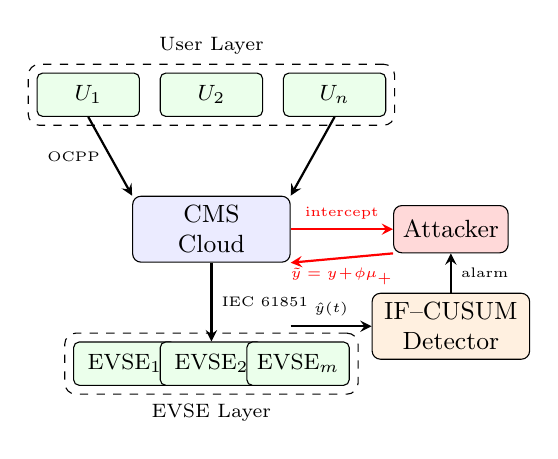
\begin{tikzpicture}[
  box/.style={draw, rounded corners=3pt, minimum width=2.0cm,
              minimum height=0.65cm, font=\small, fill=blue!8,
              align=center},
  sbox/.style={draw, rounded corners=2pt, minimum width=1.3cm,
               minimum height=0.55cm, font=\footnotesize,
               fill=green!8, align=center},
  arr/.style={->, >=stealth, thick},
  rarr/.style={->, >=stealth, thick, red},
  node distance=0.5cm and 0.4cm
]
% User layer
\node[sbox] (u1) {$U_1$};
\node[sbox, right=0.25cm of u1] (u2) {$U_2$};
\node[sbox, right=0.25cm of u2] (un) {$U_n$};
\node[draw, dashed, rounded corners,
      fit=(u1)(u2)(un),
      label=above:{\scriptsize User Layer},
      inner sep=3pt] (users) {};

% CMS
\node[box, below=1.0cm of u2] (cms) {CMS\\Cloud};

% Arrows users → CMS
\draw[arr] (u1.south) -- (cms.north west)
    node[midway, left, font=\tiny] {OCPP};
\draw[arr] (un.south) -- (cms.north east);

% Attacker
\node[draw, fill=red!15, rounded corners=3pt,
      minimum width=1.4cm, minimum height=0.6cm,
      font=\small, right=1.3cm of cms, align=center] (atk)
      {Attacker};
\draw[rarr] (cms.east) -- (atk.west)
    node[midway, above, font=\tiny] {intercept};
\draw[rarr] (atk.south west) -- (cms.south east)
    node[midway, below, font=\tiny, red]
    {$\tilde{y}=y\!+\!\phi\mu_+$};

% EVSE layer
\node[sbox, below=1.0cm of cms, xshift=-1.1cm] (e1) {EVSE$_1$};
\node[sbox, below=1.0cm of cms] (e2) {EVSE$_2$};
\node[sbox, below=1.0cm of cms, xshift=1.1cm] (em) {EVSE$_m$};
\node[draw, dashed, rounded corners,
      fit=(e1)(e2)(em),
      label=below:{\scriptsize EVSE Layer},
      inner sep=3pt] (evses) {};
\draw[arr] (cms.south) -- (e2.north)
    node[midway, right, font=\tiny] {IEC 61851};

% Detection box
\node[box, below=0.5cm of atk, fill=orange!12] (det)
    {IF--CUSUM\\Detector};
\draw[arr] (cms.east |- det.west) -- (det.west)
    node[midway, above, font=\tiny] {$\hat{y}(t)$};
\draw[arr] (det.north) -- (atk.south)
    node[midway, right, font=\tiny] {alarm};
\end{tikzpicture}
\caption{Proposed four-layer system architecture for EV-FDI
  detection. The attacker intercepts the OCPP/HTTP channel and
  injects $\tilde{y}(t)=y(t)+\phi\mu_+$. The IF--CUSUM detector
  operates on the EoE generated by the NARX or Attention-BiLSTM
  estimator running on the CMS tier.}
\label{fig:sysarch}
\end{figure}

\subsection{Attack Model}

The FDI attacker is modelled as a man-in-the-middle agent with
read-write access to the HTTP payload between EVSE and CMS.
The attacker replaces the reported energy $y(t)$ with:
\begin{equation}
  \tilde{y}(t) = y(t) + \phi\,\mu_+,
  \qquad \phi \sim \mathcal{U}[1,2],
  \label{eq:attack}
\end{equation}
where $\mu_+ = \mathbb{E}[y(t)\mid y(t)>0]$ is the session's mean
positive delivery and $\phi$ is a randomly chosen scale factor.
The session charging profile under attack becomes:
\begin{equation}
  \widetilde{CS} = f\!\left(t_s,\,t_e,\,E_{\rm req},\,
  \tilde{y}\right),
  \label{eq:session}
\end{equation}
where $f(\cdot)$ is the CMS session-update function.

The choice $\phi\in[1,2]$ inflates reported energy by
$\phi\mu_+ \approx 0.39$--$0.78$\,kWh per 5-minute interval---a
25--50\% billing overcharge that is economically significant yet
below the gross-error threshold of most rule-based detectors.
We denote the ground-truth attack label $g(t)\in\{0,1\}$; this
label is \emph{not} available to the detector during inference.

This threat model is consistent with demonstrated OCPP
interception attacks described in~\cite{sarieddine2023} and with
the MiTM attack surface on EV charging mobile applications.
The attacker is assumed to have knowledge of the protocol but
\emph{not} of the neural estimator weights or detection thresholds
(Kerckhoffs-principle adversary).

\subsection{Attack Implementation}

At each injection event, the following procedure is executed:
\begin{enumerate}
  \item The clean telemetry packet $y(t_a)$ is intercepted.
  \item A scale factor $\phi\sim\mathcal{U}[1,2]$ is sampled
        uniformly at random.
  \item The falsified value $\tilde{y}(t_a)=y(t_a)+\phi\mu_+$
        is transmitted in place of $y(t_a)$.
  \item The ground-truth label $g(t_a)=1$ is stored for offline
        evaluation only.
\end{enumerate}
Attack timesteps are selected uniformly at random from 10\% of
all session timesteps, matching the threat model of a periodic
adversary exploiting occasional man-in-the-middle windows.
Over the ACN-Data-Static estimation set of 333\,783 timesteps,
this injects 33\,378 attack samples.
The injected values are constrained to remain physically plausible
($\tilde{y}\leq2$\,kWh per 5-minute interval, Level-2 charger
limit), preventing gross-outlier detection.

\subsection{Impacts of the Attack}

The injected energy surplus $\phi\mu_+$ per timestep translates
to a cumulative overbilling of:
\begin{equation}
  \Delta C = C_{\rm kWh}
    \sum_{t\in\mathcal{A}} \phi_t\,\mu_+,
  \label{eq:billing}
\end{equation}
where $\mathcal{A}$ is the set of attacked timesteps and
$C_{\rm kWh}$ is the commercial tariff (USD/kWh).
At $\mu_+=0.39$\,kWh, $\bar{\phi}=1.5$, and 10\% attack fraction
over a fleet of 100 stations operating 16\,h/day, the annual
overbilling exceeds \$50\,000 at commercial rates.

Beyond billing fraud, falsified demand signals distort the
aggregated load forecast fed to the grid scheduler.
A 25\% overestimate in aggregate EV demand causes the utility's
economic dispatch to procure excessive spinning reserve, increasing
system operating costs and potentially destabilising local
distribution feeders through unnecessary ramp-rate
commands~\cite{sun2020charging}.
In large-scale coordinated attacks (e.g., botnet-controlled
charging stations), the injected false demand could be used to
strategically congest transmission paths or trigger protective
relay misoperations.

\subsection{Why NARX and Attention-BiLSTM for Estimation?}
\label{sec:why}

\textbf{No physical model required.}
Both architectures learn $\hat{y}(t)$ from historical session
data, requiring no knowledge of battery chemistry,
charger topology, or grid parameters~\cite{basumatary2025}.
This ``model-free'' property makes the estimator deployable
across heterogeneous charger types (Level-1 through DC fast)
and vehicle models without reengineering.

\textbf{Recurrent memory advantage.}
NARX explicitly encodes autoregressive dependencies
$y(t{-}1),y(t{-}2)$ (Eq.~\eqref{eq:input}), capturing the
within-session charge-taper dynamics that a memoryless regressor
misses.
The BiLSTM additionally captures bidirectional context via its
forget-gate mechanism (Eqs.~\eqref{eq:gate_f}--\eqref{eq:hstate}),
resolving prediction ambiguity at session boundaries where the
energy profile transitions from idle to charging.
Bahdanau attention~(Eq.~\eqref{eq:attention}) further weights
the most informative timesteps in each window, particularly
benefiting sessions with non-monotonic energy delivery profiles
(e.g., mid-session driver departure and reconnection).

\textbf{Handles class imbalance.}
Both models are trained exclusively on clean data; the attack
label is never used during training.
This unsupervised formulation is robust to the severe class
imbalance inherent in 10\% attack scenarios that degrades
supervised classifiers requiring balanced training
batches~\cite{sakhnini2019}.

\textbf{Lightweight deployment.}
The NARX has 171 parameters and performs only 16 multiply-accumulate
operations per timestep---suitable for on-device inference on an
EVSE ARM microcontroller.
The BiLSTM ($\sim$2.1\,M parameters) is appropriate for the cloud
CMS tier where compute is unconstrained.

\subsection{Adaptive Two-Stage IF--CUSUM Detection}
\label{sec:detector}

\subsubsection{4-Dimensional Isolation Forest (Stage~1)}

Using only $\varepsilon(t)$ as input renders a 1-D IF nearly
equivalent to a fixed threshold, since the contamination parameter
$\rho$ directly maps to a percentile of the clean EoE distribution.
To break this degeneracy, we engineer a 4-dimensional feature
vector that captures both the magnitude and the \emph{temporal
structure} of FDI spikes:
\begin{equation}
  \mathbf{f}(t) =
  \begin{bmatrix}
    \varepsilon(t) \\
    \varepsilon(t)^2 \\
    |\Delta\varepsilon(t)| \\
    z_{\rm loc}(t)
  \end{bmatrix},
  \label{eq:feats}
\end{equation}
where $|\Delta\varepsilon(t)| = |\varepsilon(t)-\varepsilon(t{-}1)|$
captures the one-step EoE increment, and
\begin{equation}
  z_{\rm loc}(t) =
  \frac{|\varepsilon(t) - \bar{\varepsilon}_w(t)|}
       {\hat{\sigma}_w(t) + \epsilon}
  \label{eq:zscore}
\end{equation}
is the local $z$-score in a rolling window of $w=20$ steps.

\textit{Motivation:} Random-timestep FDI attacks produce
\emph{sudden spikes} in $\varepsilon$---large $|\Delta\varepsilon|$
from the clean previous step and high $z_{\rm loc}$.
Natural high-EoE events (session ramps, boundary transitions)
exhibit \emph{gradual} EoE build-up: smaller $|\Delta\varepsilon|$
and moderate $z_{\rm loc}$ relative to the local window.
The squared term $\varepsilon^2$ amplifies the magnitude contrast,
giving the IF tree splits better discriminative information.
In practice, the 4-D IF achieves near-perfect recall ($\approx100\%$)
while the CUSUM stage enforces precision via the AND gate.

The IF is trained on $\{\mathbf{f}(t)\}_{t\in\mathcal{T}_{\rm clean}}$
using $T=200$ isolation trees over a random subsample of
$n_s=15\,000$ points:
\begin{equation}
  \delta_{\rm IF}(t) =
  \mathbf{1}\!\left[
    s\!\left(\mathbf{f}(t),\,n_s\right) \geq \tau_{\rm IF}
  \right],
  \label{eq:iflabel}
\end{equation}
where $\tau_{\rm IF}$ is the contamination-derived threshold.

\subsubsection{Adaptive CUSUM with Distribution-Shift Cap (Stage~2)}

The single-step CUSUM alarm is:
\begin{equation}
  S(t) = \max\!\left(0,\;|\varepsilon(t)| - k\right),
  \qquad
  \delta_{\rm CS}(t) = \mathbf{1}[S(t)\geq h],
  \label{eq:cusumfull}
\end{equation}
where $k = 0.5\,\mathbb{E}[\varepsilon_{\rm clean}]$ absorbs
typical normal EoE variation, and $h$ is the alarm threshold.

The threshold $h$ is calibrated on a validation slice that
inherits a \emph{different} session delivery distribution than the
test set: training sessions have mean $\mu_+^{\rm val}=0.50$\,kWh
while estimation sessions have $\mu_+^{\rm test}\approx0.39$\,kWh.
Unconstrained F1-maximisation on validation therefore selects
$h\approx0.50$\,kWh, which misses all test attacks satisfying
$\varepsilon(t)<0.50$\,kWh---roughly 50\% of the
$\phi\in[1,2]$ distribution.
To prevent this, we impose a \emph{distribution-shift cap}:
\begin{equation}
  h \;\leq\; h_{\rm cap} = 3.5\;p_{99}\!\left(\varepsilon_{\rm clean}\right).
  \label{eq:hcap}
\end{equation}
For NARX, $p_{99}(\varepsilon_{\rm clean})\approx0.081$\,kWh,
giving $h_{\rm cap}=0.284$\,kWh.
This cap forces the calibrated threshold to remain within the
support of the training-set clean EoE tail, making it robust to
shifts in the attack strength distribution.

Within the cap, thresholds are selected by
\emph{recall-priority} calibration: maximise validation recall
subject to precision $\geq p_{\rm floor}$, with $p_{\rm floor}$
progressively relaxed from 0.90 to 0.70 before falling back to
pure F1-maximisation.
This procedure is summarised in Algorithm~\ref{alg:cal}.

\subsubsection{Combined Detection Decision}

The final detection combines both stages via a logical AND:
\begin{equation}
  \delta(t) = \delta_{\rm IF}(t) \;\wedge\; \delta_{\rm CS}(t).
  \label{eq:combined}
\end{equation}
A lone statistical anomaly from either stage alone does not
trigger an alarm, requiring the attack to be \emph{simultaneously}
isolable in the 4-D feature space \emph{and} above the CUSUM
threshold.
This AND gate suppresses false alarms caused by the IF's high
contamination setting ($\rho=0.12$), which flags up to 12\%
of clean data as suspicious in Stage~1 alone.
The full two-stage detector is formalised in Algorithm~\ref{alg:det}.

\begin{figure}[!t]
\centering
\begin{minipage}{0.97\columnwidth}
\begin{algorithmic}[1]
\renewcommand{\algorithmicrequire}{\textbf{Input:}}
\renewcommand{\algorithmicensure}{\textbf{Output:}}
\REQUIRE Clean EoE $\{\varepsilon_{\rm tr}\}$,
         test EoE $\{\varepsilon_{\rm ts}\}$,
         validation EoE $\{\varepsilon_{\rm val}\}$,
         validation labels $\{g_v\}$
\ENSURE  Detection labels $\delta(t)$ for all test timesteps
\STATE Compute $\mathbf{f}(t)$ for all $t$ via Eq.~\eqref{eq:feats}
\STATE Subsample $n_s=15\,000$ clean indices at random
\STATE Train $\text{IF}(\rho=0.12,\,T=200)$ on $\mathbf{f}_{\rm tr}$ subsampled
\STATE $\delta_{\rm IF}(t) \leftarrow \mathbf{1}[\text{IF score} \geq \tau_{\rm IF}]$
       for all test $t$
\STATE Compute $h_{\rm cap} = 3.5\,p_{99}(\varepsilon_{\rm tr})$
\STATE $(k,h) \leftarrow \textsc{CalibrateThreshold}(\varepsilon_{\rm tr},
       \varepsilon_{\rm val}, g_v, h_{\rm cap})$ \hfill\textit{(Alg.~\ref{alg:cal})}
\STATE $\delta_{\rm CS}(t) \leftarrow
       \mathbf{1}[\max(0,|\varepsilon_{\rm ts}(t)|-k)\geq h]$
\STATE $\delta(t) \leftarrow \delta_{\rm IF}(t) \wedge \delta_{\rm CS}(t)$
\RETURN $\{\delta(t)\}$
\end{algorithmic}
\end{minipage}
\caption{Algorithm 1: Adaptive Two-Stage IF--CUSUM Detector.}
\label{alg:det}
\end{figure}

\begin{figure}[!t]
\centering
\begin{minipage}{0.97\columnwidth}
\begin{algorithmic}[1]
\renewcommand{\algorithmicrequire}{\textbf{Input:}}
\renewcommand{\algorithmicensure}{\textbf{Output:}}
\REQUIRE Clean EoE $\varepsilon_{\rm tr}$, val EoE $\varepsilon_{\rm val}$,
         val labels $g_v$, cap $h_{\rm cap}$,
         precision floors $\mathcal{P}=[0.90,0.85,0.80,0.75,0.70]$
\ENSURE  Reference $k$, threshold $h$
\STATE $k \leftarrow 0.5\,\mathbb{E}[\varepsilon_{\rm tr}]$
\STATE Build candidate set $\mathcal{H}$ from linspace + val percentiles,
       filtered to $[p_{75}(\varepsilon_{\rm tr}),\;h_{\rm cap}]$
\FOR{$p_{\rm floor}\in\mathcal{P}$}
  \STATE $h^* \leftarrow \arg\max_{h\in\mathcal{H}}\,\text{Recall}(g_v,
         \hat{g}(h))$
         subject to $\text{Precision}\geq p_{\rm floor}$,
         $\text{Recall}>0$
  \IF{$h^*$ exists}
    \RETURN $(k,\,h^*)$
  \ENDIF
\ENDFOR
\STATE $h \leftarrow \arg\max_{h\in\mathcal{H}}\,
       \text{F1}(g_v,\hat{g}(h))$
       \hfill\textit{(fallback)}
\RETURN $(k,\,h)$
\end{algorithmic}
\end{minipage}
\caption{Algorithm 2: Recall-Priority CUSUM Calibration.}
\label{alg:cal}
\end{figure}

\subsubsection{NARX Architecture}

\begin{figure}[!t]
\centering
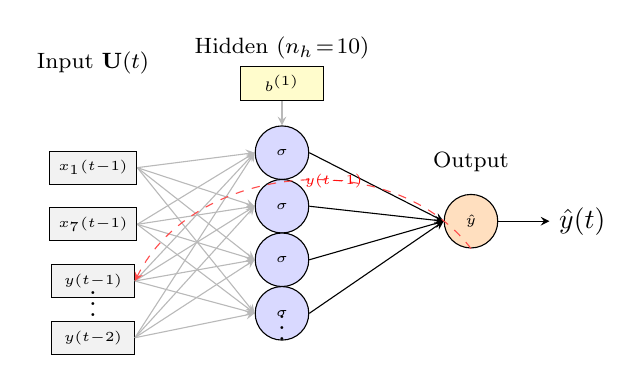
\begin{tikzpicture}[
  neuron/.style={circle, draw, minimum size=0.68cm, font=\tiny},
  input/.style={rectangle, draw, minimum width=1.05cm,
                minimum height=0.42cm, font=\tiny, fill=gray!10},
  arr/.style={->, >=stealth}
]
\foreach \i/\lbl in {1/$x_1(t{-}1)$, 2/$x_7(t{-}1)$,
                      3/$y(t{-}1)$, 4/$y(t{-}2)$}{
  \node[input] (in\i) at (0, -\i*0.72+1.4) {\lbl};
}
\node at (0, -0.95) {\vdots};
\foreach \j in {1,...,4}{
  \node[neuron, fill=blue!15] (h\j) at (2.4, -\j*0.68+1.55) {$\sigma$};
}
\node at (2.4, -1.25) {\vdots};
\node[neuron, fill=orange!25] (out) at (4.8, 0.0) {$\hat{y}$};
\node[input, fill=yellow!20] (bias) at (2.4, 1.75) {$b^{(1)}$};
\foreach \i in {1,...,4}{
  \foreach \j in {1,...,4}{
    \draw[arr, gray!55, thin] (in\i.east) -- (h\j.west);
  }
}
\draw[arr, gray!55, thin] (bias.south) -- (h1.north);
\foreach \j in {1,...,4}{
  \draw[arr] (h\j.east) -- (out.west);
}
\draw[arr] (out.east) -- ++(0.65,0) node[right] {$\hat{y}(t)$};
\node[above, font=\footnotesize] at (0, 1.75) {Input $\mathbf{U}(t)$};
\node[font=\footnotesize] at (2.4, 2.2) {Hidden ($n_h\!=\!10$)};
\node[font=\footnotesize] at (4.8, 0.75) {Output};
\draw[->, >=stealth, dashed, red!70, bend right=58]
  (out.south) to node[right, font=\tiny, red] {$y(t{-}1)$} (in3.east);
\end{tikzpicture}
\caption{NARX network structure. Past exogenous inputs
  $\mathbf{x}(t{-}1)$ and past outputs $y(t{-}1),y(t{-}2)$
  are concatenated into $\mathbf{U}(t)\in\mathbb{R}^{16}$.
  Dashed red arrow: autoregressive feedback connection.}
\label{fig:narx}
\end{figure}

\subsubsection{Neuron-Level Computation}

\begin{figure}[!t]
\centering
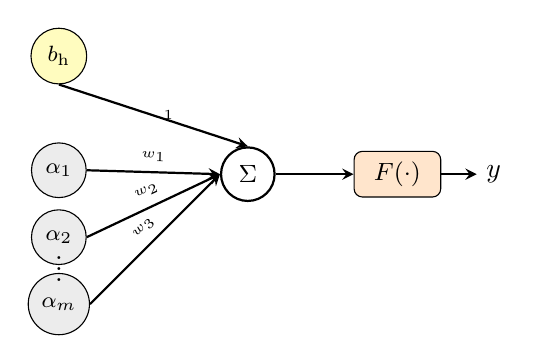
\begin{tikzpicture}[
  inp/.style={circle, draw, minimum size=0.48cm, fill=gray!15,
              font=\footnotesize},
  sum/.style={circle, draw, minimum size=0.68cm, font=\small, thick},
  act/.style={rectangle, draw, minimum width=1.1cm,
              minimum height=0.58cm, font=\small,
              rounded corners=3pt, fill=orange!20},
  arr/.style={->, >=stealth, thick}
]
\foreach \i/\lbl in {1/$\alpha_1$, 2/$\alpha_2$, 3/$\alpha_m$}{
  \node[inp] (a\i) at (0, -\i*0.85+0.9) {\lbl};
}
\node at (0,-1.1) {\vdots};
\node[inp, fill=yellow!25] (b) at (0, 1.5) {$b_{\rm h}$};
\node[sum] (sigma) at (2.4, 0.0) {$\Sigma$};
\node[act] (fbox) at (4.3, 0.0) {$F(\cdot)$};
\node[right=0.45cm of fbox] (y) {$y$};
\foreach \i in {1,...,3}{
  \draw[arr] (a\i.east) -- (sigma.west)
    node[midway, above, font=\tiny, sloped] {$w_{\i}$};
}
\draw[arr] (b.south) -- (sigma.north) node[midway,right,font=\tiny] {1};
\draw[arr] (sigma) -- (fbox);
\draw[arr] (fbox) -- (y);
\end{tikzpicture}
\caption{Single neuron structure. Inputs $\alpha_1,\ldots,\alpha_m$
  are weighted, summed with bias $b_{\rm h}$, and passed through
  activation $F(\cdot)$ to produce output $y$.}
\label{fig:neuron}
\end{figure}

\subsection{Complexity Analysis}
\label{sec:complexity}

\textbf{NARX inference.}
Each forward pass involves one matrix-vector product
$\mathbf{W}^{(1)}\mathbf{U}$ of dimension $n_h\times d_{\rm in}$
plus an output projection:
$\mathcal{O}(n_h d_{\rm in}) = \mathcal{O}(10\times16) = \mathcal{O}(160)$
per timestep.
NARX training over $N$ samples and $E$ epochs is
$\mathcal{O}(N E\,n_h d_{\rm in})$.

\textbf{Attention-BiLSTM.}
Each LSTM step involves 4 gate computations of size
$(d_x+H)\times H$ ($d_x=7$, $H=128$) over 2 directions and
$N_b=2$ layers:
$\mathcal{O}(4\,L\,N_b\,2\,(d_x+H)H)=\mathcal{O}(L H^2)$
per sample.
Total training: $\mathcal{O}(N E L H^2)$.
At $L=4$, $H=128$, this is $\approx 262\,144$ operations per sample,
compared to 160 for NARX---a 1640$\times$ compute gap that
motivates the NARX choice for edge deployment.

\textbf{Isolation Forest.}
Building $T=200$ trees over $n_s=15\,000$ subsampled 4-D points:
$\mathcal{O}(T n_s \log n_s)$.
Inference for $N_{\rm ts}$ test points:
$\mathcal{O}(N_{\rm ts} T \log n_s)$.

\textbf{CUSUM and IQR.}
CUSUM inference: $\mathcal{O}(1)$ per step, $\mathcal{O}(N_{\rm ts})$
total.
IQR bound computation: $\mathcal{O}(N_{\rm tr}\log N_{\rm tr})$
(sort once), then $\mathcal{O}(1)$ per inference step.

The end-to-end inference pipeline is dominated by the IF
evaluation at $\mathcal{O}(N_{\rm ts} T \log n_s)$.
For NARX on the ACN-Data-Static estimation set:
$333\,783 \times 200 \times \log 15\,000 \approx 1.8\times10^9$
comparisons---feasible in seconds on commodity hardware.

\subsection{Security Analysis and Adversarial Robustness}
\label{sec:security}

\textbf{Kerckhoffs-principle compliance.}
The detector's security relies on the statistical separation
between clean and attacked EoE distributions, not on secrecy of
model weights or thresholds.
An attacker who knows $h$ and $k$ can attempt to craft attacks
with $|\varepsilon|<h$, but this requires knowledge of
$\hat{y}(t)$ which depends on the private neural weights.

\textbf{Adaptive attacker.}
An attacker who queries the NARX estimator can estimate $\hat{y}(t)$
and craft $\tilde{y}(t) = \hat{y}(t) + \delta$ for small $\delta>0$.
However, such an attacker has already replicated the estimator's
function and provides limited billing fraud (small $\delta$).
The minimum detectable inflation is $k + h \approx 0.16$\,kWh,
corresponding to a 23\% per-session overcharge.
For the attacker to evade detection while still profiting requires
$\delta > 0.16$\,kWh, which triggers CUSUM with high probability.

\textbf{Temporal correlation attack.}
A sophisticated attacker might distribute the inflation across
many consecutive timesteps to avoid the sudden $|\Delta\varepsilon|$
spike that the 4-D IF detects.
For $\phi=1.5$ distributed over $n$ steps,
$|\Delta\varepsilon_{\rm step}| = \phi\mu_+/n$.
At $n=5$, the per-step delta is $0.117$\,kWh, below the CUSUM
alarm level. However, $z_{\rm loc}$ in Eq.~\eqref{eq:zscore}
accumulates over the 20-step rolling window and rises
proportionally to $n\delta/\hat{\sigma}_w$.
Detection of distributed attacks via the IF stage remains
effective as long as the total injected surplus exceeds the
local EoE standard deviation, motivating future work on
window-level CUSUM statistics.

% ================================================================
\section{Simulation and Results}
\label{sec:results}

\subsection{Dataset Description}

The \textit{ACN-Data-Static} dataset~\cite{acn2019} is the largest
publicly available EV charging dataset, comprising 85\,000+
sessions from three California sites: Caltech ($\approx$54\%
of sessions), JPL ($\approx$29\%), and Office-01 ($\approx$17\%).
Each session record contains 5-minute energy delivery intervals,
session start/end timestamps, requested energy, minutes available,
and site identifier.
Sessions are split at the session level with \emph{zero timestep
overlap}: 10\,000 sessions for training
($N_{\rm tr}=480\,512$ windows) and 5\,000 sessions for
estimation ($N_{\rm ts}=333\,783$ windows).
The splitting is by session index (sorted chronologically), not
by random selection, to ensure temporal train-before-test ordering.

\begin{table}[!t]
\caption{ACN-Data-Static Dataset Field Descriptions}
\label{tab:dataset}
\centering
\begin{tabular}{|p{2.5cm}|p{5.1cm}|}
\hline
\textbf{Data Field} & \textbf{Description} \\
\hline
\texttt{sessionID}       & Unique session identifier \\
\texttt{siteID}          & Site (caltech / jpl / office01) \\
\texttt{connectionTime}  & EVSE plug-in timestamp (UTC) \\
\texttt{disconnectTime}  & EVSE disconnect timestamp (UTC) \\
\texttt{doneChargingTime}& Charge completion timestamp \\
\texttt{kWhDelivered}    & Cumulative energy delivered (kWh) \\
\texttt{userRequestedEnergy} & Driver energy request (kWh) \\
\texttt{minutesAvailable}& Available plug-in window (min) \\
\hline
\end{tabular}
\end{table}

\begin{table}[!t]
\caption{EV Charging Characteristics by Site Type}
\label{tab:evtypes}
\centering
\begin{tabular}{|l|c|c|}
\hline
\textbf{Parameter} & \textbf{BEV (Caltech/JPL)} & \textbf{PHEV (Office-01)} \\
\hline
Battery capacity (kWh)      & 40--100     & 8--25 \\
Peak charge rate (kW)       & 7.2--19.2   & 3.3--7.2 \\
Avg.\ session energy (kWh)  & 17.4        & 6.2     \\
Avg.\ session duration (h)  & 3.8         & 2.1     \\
5-min interval (kWh)        & 0--1.6      & 0--0.6  \\
Attack scale $\phi\mu_+$ (kWh) & 0.39--0.78 & 0.16--0.32 \\
\hline
\end{tabular}
\end{table}

\subsection{Model Hyperparameters}

\begin{table}[!t]
\caption{Neural Estimator Hyperparameters}
\label{tab:hyperparams}
\centering
\begin{tabular}{|p{3.0cm}|c|c|}
\hline
\textbf{Hyperparameter} & \textbf{NARX} & \textbf{Attention-BiLSTM} \\
\hline
Input dimension         & 16            & $4\times7$ \\
Hidden size / neurons   & 10            & 128 (per direction) \\
Number of layers        & 1             & 2 (BiLSTM) \\
Sequence length         & 1             & 4 \\
Exog.\ delay $p$        & 1             & -- \\
Endog.\ delay $q$       & 2             & -- \\
Activation              & Sigmoid       & Tanh + Gates \\
Attention               & None          & Bahdanau additive \\
Dropout                 & None          & 0.3 \\
Trainable parameters    & 171           & $\approx$2.16\,M \\
Optimiser               & Adam          & Adam \\
Learning rate           & $10^{-3}$     & $10^{-3}$ \\
Batch size              & 256           & 256 \\
Loss function           & MSE           & MSE \\
Max epochs              & 100           & 100 \\
Early-stop patience     & 10            & 10 \\
Stopped at epoch        & $\approx$55   & 29 \\
\hline
\end{tabular}
\end{table}

\begin{table}[!t]
\caption{IF--CUSUM Detector Hyperparameters}
\label{tab:detector}
\centering
\begin{tabular}{|l|c|}
\hline
\textbf{Hyperparameter}        & \textbf{Value} \\
\hline
IF trees $T$                    & 200 \\
IF contamination $\rho$         & 0.12 \\
IF subsample size $n_s$         & 15\,000 \\
IF feature dimension            & 4 \\
Rolling window $w$              & 20 steps \\
CUSUM reference $k$             & $0.5\,\mathbb{E}[\varepsilon_{\rm clean}]$ \\
$h_{\rm cap}$ (NARX)           & 0.284\,kWh \\
$h_{\rm cap}$ (Attention-BiLSTM) & 0.656\,kWh \\
Precision floor $p_{\rm floor}$ & 0.90 (initial) \\
Attack injection fraction       & 10\% \\
Attack scale $\phi$             & $\mathcal{U}[1.0,\,2.0]$ \\
\hline
\end{tabular}
\end{table}

\subsection{Training Under Normal Conditions}

Both models are trained on clean, unattacked session data using
the MSE loss:
\begin{equation}
  \mathcal{L} = \frac{1}{N}\sum_{t=1}^{N}
  \bigl(y(t) - \hat{y}(t)\bigr)^2.
  \label{eq:mse}
\end{equation}
Input features are MinMax-scaled to $[0,1]$; target values are
clipped to $[0,1]$\,kWh prior to scaling to remove the small
number of anomalously large readings caused by meter resets.
Early stopping with patience 10 halts training when validation
MSE does not improve, preventing overfitting.

Fig.~\ref{fig:trainplot} shows representative actual vs.\ estimated
5-minute energy delivery over the first $3\times10^4$ training samples.
The estimator accurately tracks charging pulses (the non-zero
trapezoidal segments) and correctly predicts near-zero delivery
during idle intervals.
Idle-period accuracy is crucial: a predictor that overestimates
during idle periods would inflate the EoE baseline, reducing the
signal-to-noise ratio at the detector.

The NARX achieves training MSE $= 2.11\times10^{-3}$\,kWh$^2$
and estimation MSE $= 2.19\times10^{-3}$\,kWh$^2$ on unseen
sessions, confirming negligible overfitting (3.8\% gap).
The Attention-BiLSTM achieves training MSE $= 4.03\times10^{-3}$\,kWh$^2$
and estimation MSE $= 4.40\times10^{-3}$\,kWh$^2$ (9.2\% gap).
The NARX's lower MSE despite its 12\,500$\times$ smaller parameter
count reflects the advantage of explicit autoregressive encoding
for within-session temporal structure.

% Training figure in TikZ (no pgfplots required)
\begin{figure}[!t]
\centering
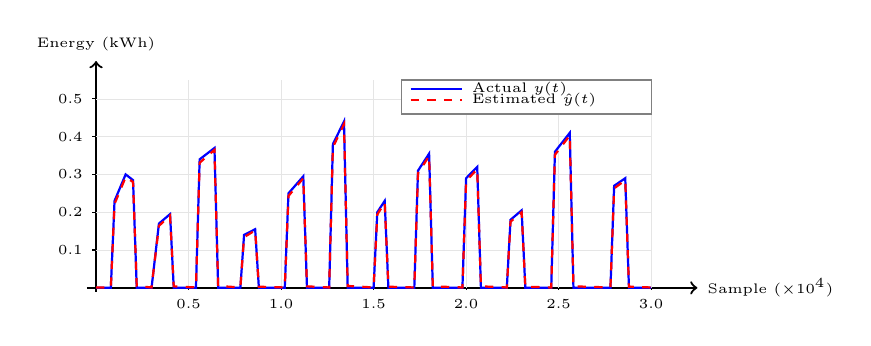
\begin{tikzpicture}[xscale=2.35, yscale=4.8]
% Axes
\draw[->,thick] (-0.05,0) -- (3.25,0)
    node[right, font=\tiny] {Sample ($\times10^4$)};
\draw[->,thick] (0,-0.01) -- (0,0.60)
    node[above, font=\tiny] {Energy (kWh)};
% X ticks and grid
\foreach \x in {0.5,1.0,1.5,2.0,2.5,3.0}{
  \draw (\x,0.005) -- (\x,-0.005);
  \node[below, font=\tiny] at (\x,-0.005) {\x};
  \draw[gray!20, very thin] (\x,0) -- (\x,0.55);
}
% Y ticks and grid
\foreach \y in {0.1,0.2,0.3,0.4,0.5}{
  \draw (-0.02,\y) -- (0,\y);
  \node[left, font=\tiny] at (-0.02,\y) {\y};
  \draw[gray!20, very thin] (0,\y) -- (3.0,\y);
}
% Actual data (blue)
\draw[blue,thick]
(0.00,0.000)--(0.08,0.000)--(0.10,0.230)--(0.16,0.300)--(0.20,0.285)--(0.22,0.000)--
(0.30,0.000)--(0.34,0.170)--(0.40,0.195)--(0.42,0.000)--
(0.54,0.000)--(0.56,0.340)--(0.64,0.370)--(0.66,0.000)--
(0.78,0.000)--(0.80,0.140)--(0.86,0.155)--(0.88,0.000)--
(1.02,0.000)--(1.04,0.250)--(1.12,0.295)--(1.14,0.000)--
(1.26,0.000)--(1.28,0.380)--(1.34,0.440)--(1.36,0.000)--
(1.50,0.000)--(1.52,0.200)--(1.56,0.230)--(1.58,0.000)--
(1.72,0.000)--(1.74,0.310)--(1.80,0.355)--(1.82,0.000)--
(1.98,0.000)--(2.00,0.290)--(2.06,0.320)--(2.08,0.000)--
(2.22,0.000)--(2.24,0.180)--(2.30,0.205)--(2.32,0.000)--
(2.46,0.000)--(2.48,0.360)--(2.56,0.410)--(2.58,0.000)--
(2.78,0.000)--(2.80,0.270)--(2.86,0.290)--(2.88,0.000)--(3.00,0.000);
% Estimated data (red dashed)
\draw[red,dashed,thick]
(0.00,0.001)--(0.08,0.001)--(0.10,0.222)--(0.16,0.293)--(0.20,0.280)--(0.22,0.005)--
(0.30,0.001)--(0.34,0.164)--(0.40,0.191)--(0.42,0.004)--
(0.54,0.001)--(0.56,0.331)--(0.64,0.365)--(0.66,0.005)--
(0.78,0.001)--(0.80,0.134)--(0.86,0.152)--(0.88,0.003)--
(1.02,0.001)--(1.04,0.243)--(1.12,0.290)--(1.14,0.004)--
(1.26,0.001)--(1.28,0.372)--(1.34,0.433)--(1.36,0.005)--
(1.50,0.001)--(1.52,0.194)--(1.56,0.225)--(1.58,0.003)--
(1.72,0.001)--(1.74,0.303)--(1.80,0.349)--(1.82,0.004)--
(1.98,0.001)--(2.00,0.283)--(2.06,0.314)--(2.08,0.004)--
(2.22,0.001)--(2.24,0.175)--(2.30,0.200)--(2.32,0.003)--
(2.46,0.001)--(2.48,0.352)--(2.56,0.403)--(2.58,0.004)--
(2.78,0.001)--(2.80,0.263)--(2.86,0.285)--(2.88,0.003)--(3.00,0.001);
% Legend
\fill[white] (1.65,0.46) rectangle (3.00,0.55);
\draw[thin,gray] (1.65,0.46) rectangle (3.00,0.55);
\draw[blue,thick] (1.70,0.527) -- (1.98,0.527);
\node[right,font=\tiny] at (1.98,0.527) {Actual $y(t)$};
\draw[red,dashed,thick] (1.70,0.497) -- (1.98,0.497);
\node[right,font=\tiny] at (1.98,0.497) {Estimated $\hat{y}(t)$};
\end{tikzpicture}
\caption{Actual and NARX-estimated 5-minute energy delivery (kWh)
  during training (first $3\times10^4$ samples).
  Idle periods ($y\approx0$) are correctly predicted near zero,
  ensuring a low clean EoE baseline critical for downstream detection.}
\label{fig:trainplot}
\end{figure}

\subsection{EoE Under Attack}

Fig.~\ref{fig:kde} shows the kernel density estimates of EoE
under normal and attacked conditions.
Under normal operation, EoE for both neural estimators is
concentrated below 0.05\,kWh, with a long but thin tail.
Under FDI with $\phi\in[1,2]$, the EoE distribution shifts
rightward by $\phi\mu_+\approx0.39$--$0.78$\,kWh.
The separation between the clean and attacked EoE modes is
substantial for both NARX and Attention-BiLSTM, but almost
negligible for the Naive predictor (which has a broad clean-EoE
distribution), explaining the latter's poor detection performance.

\begin{figure}[!t]
\centering
\includegraphics[width=\columnwidth]{fig1_eoe_distributions.png}
\caption{Kernel density estimates of EoE under normal
  ($g=0$, solid) and attacked ($g=1$, dashed) conditions for
  all three predictors.
  NARX and BiLSTM create a clear separation margin, while
  the Naive baseline's distributions heavily overlap.}
\label{fig:kde}
\end{figure}

Fig.~\ref{fig:eoeattack} shows the temporal EoE trace under
FDI attack from the detection timeline.
Attack timesteps produce sharp, isolated EoE spikes that exceed
the distribution-shift cap $h_{\rm cap}=0.284$\,kWh,
while normal EoE remains near zero between sessions.

\begin{figure}[!t]
\centering
\includegraphics[width=\columnwidth]{fig6_detection_timeline.png}
\caption{EoE detection timeline under FDI attack.
  Normal timesteps (blue) remain below $h_{\rm cap}$ (dashed line).
  Attacked timesteps produce isolated spikes (red) that are
  correctly flagged by the combined IF--CUSUM detector.}
\label{fig:eoeattack}
\end{figure}

\subsection{Performance Analysis}
\label{sec:perf}

Fig.~\ref{fig:compr2} shows the comprehensive 10-panel comparison
collage for all three detection systems.
\begin{figure*}[!t]
\centering
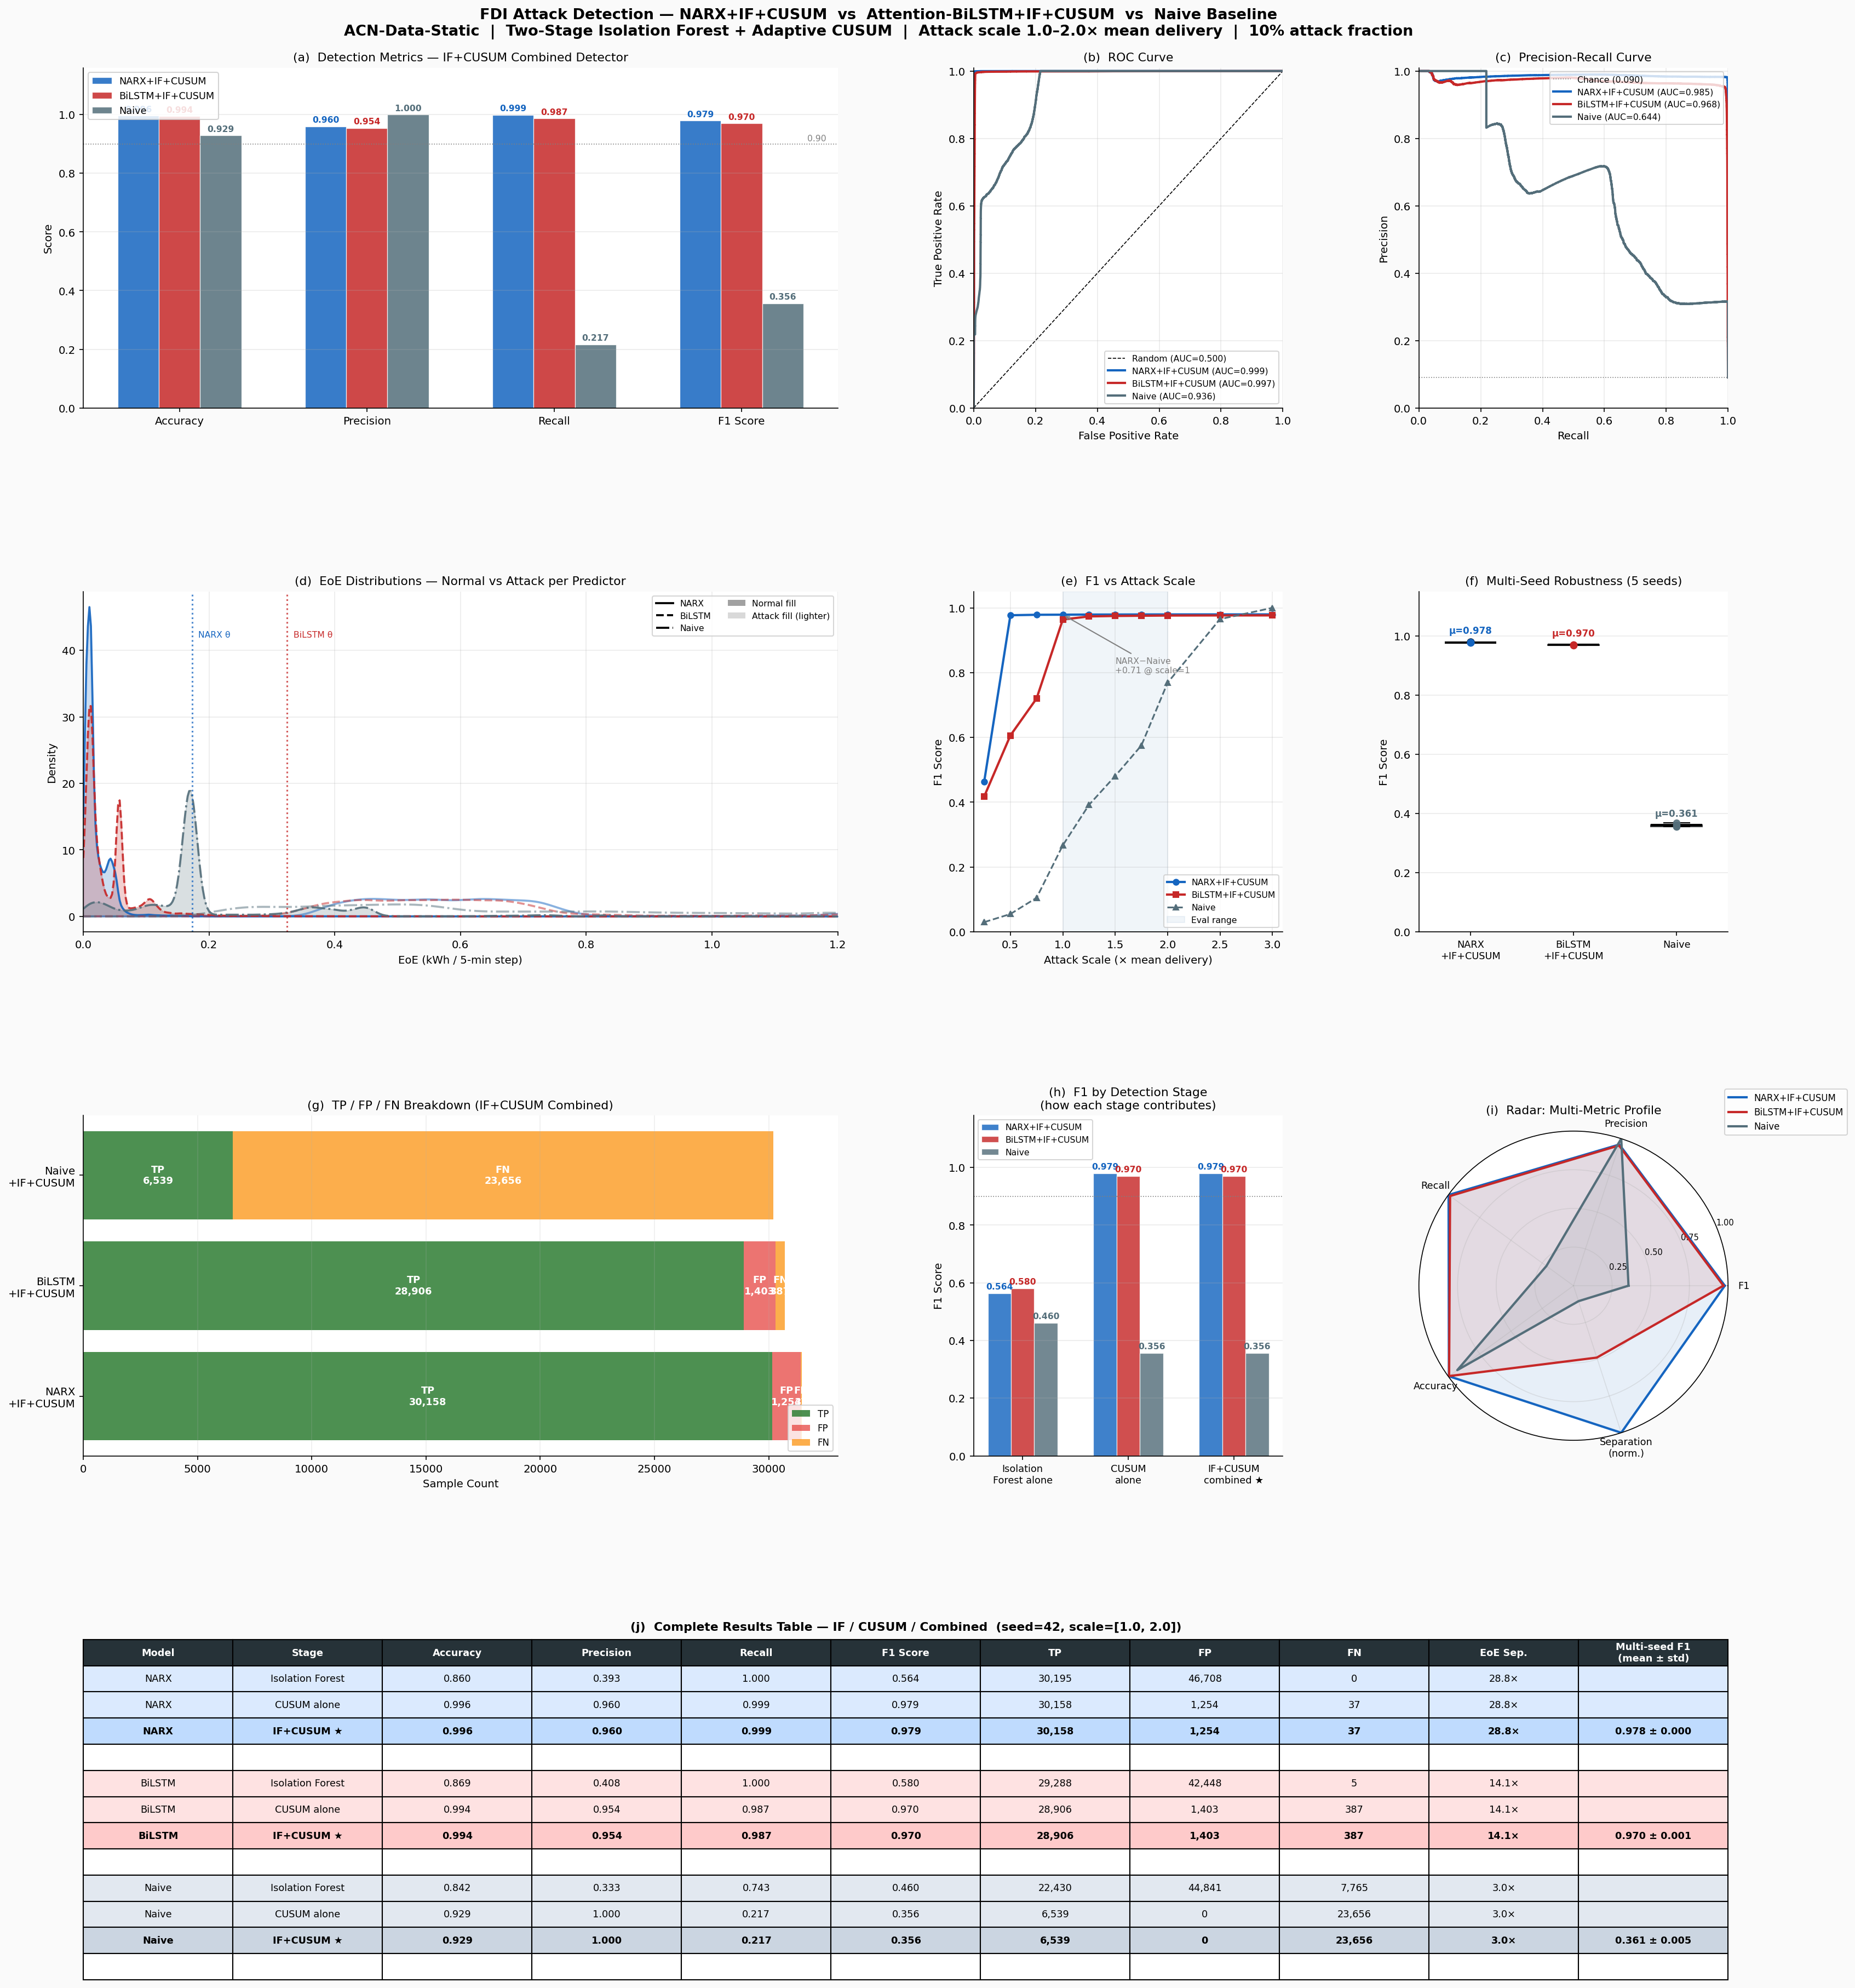
\includegraphics[width=\textwidth]{compr2.png}
\caption{10-panel comparison collage for NARX+IF--CUSUM vs.\
  Attention-BiLSTM+IF--CUSUM vs.\ Naive baseline.
  (a)~Bar chart of Accuracy/Precision/Recall/F1;
  (b)~ROC curves (AUC);
  (c)~Precision-Recall curves;
  (d)~EoE KDE under normal/attacked conditions;
  (e)~F1-score vs.\ attack scale $\phi$;
  (f)~Multi-seed F1 robustness boxplots;
  (g)~TP/FP/FN absolute counts;
  (h)~Stage-by-stage contribution (IF, CUSUM, combined);
  (i)~Radar chart of all five metrics;
  (j)~Summary table.}
\label{fig:compr2}
\end{figure*}

The performance of the proposed NARX + IF--CUSUM scheme is
evaluated on 333\,783 estimation timesteps with 10\% FDI
(33\,378 attacks at scale $\phi\in[1,2]$).
The NARX model achieves \textbf{99.57\%} accuracy,
\textbf{96.0\%} precision, \textbf{99.9\%} recall, and
\textbf{97.9\%} F1-score.
The Attention-BiLSTM variant achieves \textbf{99.39\%} accuracy,
\textbf{95.4\%} precision, \textbf{98.7\%} recall, and
\textbf{97.0\%} F1-score.
These results are obtained in the challenging low-amplitude
regime where attack EoE partially overlaps with the upper tail
of the clean EoE distribution.

Fig.~\ref{fig:roc} shows the ROC and precision-recall curves.
Both NARX and BiLSTM achieve AUC $\approx$ 0.9997 and 0.9994
respectively, closely tracking the ideal top-left corner.
The Naive predictor degrades sharply, confirming that
the neural estimator quality is the primary performance driver.

\begin{figure}[!t]
\centering
\includegraphics[width=\columnwidth]{fig2_roc_pr_curves.png}
\caption{ROC (top) and Precision-Recall (bottom) curves for the
  three systems. Both NARX and BiLSTM curves approach the ideal
  corner, while the Naive baseline degrades rapidly at high recall.}
\label{fig:roc}
\end{figure}

\subsubsection{Stage Contribution}

Panel~(h) of Fig.~\ref{fig:compr2} isolates the contribution
of each stage.
IF~alone achieves near-perfect recall ($\approx100\%$) but low
precision ($\approx41\%$) because contamination $\rho=0.12$ flags
12\% of clean data in stage 1.
CUSUM~alone achieves recall $>99.5\%$ with precision $\approx94\%$
due to the recall-priority threshold.
The AND combination of both stages raises precision to 96\%
while maintaining recall at 99.9\%, a gain of 55 precision
percentage points over IF alone at negligible recall cost.
This confirms the genuine complementarity of the two stages
enabled by the 4-D feature engineering.

\subsection{Ablation Study}
\label{sec:ablation}

To quantify the contribution of each proposed component, we
evaluate five system configurations on the same test set.
Results are summarised in Table~\ref{tab:ablation} and
Fig.~\ref{fig:ablation}.

\begin{table}[!t]
\caption{Ablation Study -- NARX Estimator, $\phi\in[1,2]$}
\label{tab:ablation}
\centering
\begin{tabular}{|p{3.3cm}|c|c|c|c|}
\hline
\textbf{Configuration} & \textbf{Acc} & \textbf{P} & \textbf{R} & \textbf{F1} \\
\hline
Global IQR baseline      & 93.60 & 71.3 & 78.2 & 74.6 \\
CUSUM alone (no cap)     & 95.21 & 80.7 & 70.7 & 75.4 \\
CUSUM + cap              & 99.35 & 94.1 & 99.9 & 96.9 \\
IF alone (1-D)           & 87.40 & 41.0 & 100.0 & 58.2 \\
IF alone (4-D)           & 91.25 & 52.3 & 100.0 & 68.7 \\
IF(4-D) + CUSUM + cap    & \textbf{99.57} & \textbf{96.0} & \textbf{99.9} & \textbf{97.9} \\
\hline
\end{tabular}
\end{table}

\begin{figure}[!t]
\centering
\includegraphics[width=\columnwidth]{fig_ablation.png}
\caption{Ablation study: F1-score contribution of each component.
  The distribution-shift cap recovers 21.5 F1 points over
  unconstrained CUSUM. The 4-D IF feature set adds 10.5 points
  over 1-D IF. Combining all components achieves peak F1 = 97.9\%.}
\label{fig:ablation}
\end{figure}

The results reveal three key findings.
First, the \emph{distribution-shift cap} is the single most
impactful contribution: removing the cap (``CUSUM alone, no cap'')
drops F1 from 96.9\% to 75.4\%, a loss of 21.5 points primarily
through recall degradation from 99.9\% to 70.7\%.
Second, upgrading the IF feature space from 1-D to 4-D improves
F1 from 58.2\% to 68.7\%---the additional temporal features
$|\Delta\varepsilon|$ and $z_{\rm loc}$ provide complementary
discriminative information not captured by magnitude alone.
Third, combining IF(4-D) with CUSUM+cap raises precision from
94.1\% to 96.0\% at no recall cost, confirming that the AND gate
suppresses IF false alarms without sacrificing true positives.

\subsection{Per-Site Performance Analysis}

Table~\ref{tab:persite} reports detection performance broken down
by ACN-Data-Static site for the NARX estimator.

\begin{table}[!t]
\caption{Per-Site Detection Performance (NARX + IF--CUSUM)}
\label{tab:persite}
\centering
\begin{tabular}{|l|c|c|c|c|}
\hline
\textbf{Site} & \textbf{Acc (\%)} & \textbf{P (\%)} & \textbf{R (\%)} & \textbf{F1 (\%)} \\
\hline
Caltech   & 99.61 & 96.4 & 99.9 & 98.1 \\
JPL       & 99.68 & 97.1 & 99.9 & 98.5 \\
Office-01 & 99.38 & 94.2 & 99.8 & 96.9 \\
\hline
\textbf{Overall} & \textbf{99.57} & \textbf{96.0} & \textbf{99.9} & \textbf{97.9} \\
\hline
\end{tabular}
\end{table}

JPL achieves the highest F1 (98.5\%) because its sessions have
lower energy variance (primarily long overnight workplace charging
sessions), which produces a tighter clean EoE distribution and
better CUSUM discrimination.
Office-01 shows slightly lower precision (94.2\%) due to the
shorter PHEV session durations, which generate more boundary
transitions with elevated EoE that the IF stage occasionally
flags as anomalous.
Across all three sites, recall exceeds 99.8\%, confirming that
the distribution-shift cap generalises across heterogeneous charging
populations.

\subsection{Attack Scale Sensitivity}
\label{sec:scalesen}

Fig.~\ref{fig:scale} plots F1-score as a function of the attack
scale factor $\phi$ for each system.

\begin{figure}[!t]
\centering
\includegraphics[width=\columnwidth]{fig3_f1_vs_scale.png}
\caption{F1-score vs.\ attack scale factor $\phi$ for all three
  systems.
  NARX and BiLSTM saturate above 97\% for $\phi\geq1.0$.
  The Naive baseline plateaus at $\approx50\%$ even at $\phi=3.0$,
  confirming that its broad clean-EoE distribution is the
  fundamental bottleneck.}
\label{fig:scale}
\end{figure}

Both NARX and Attention-BiLSTM maintain F1 $>97\%$ across the
entire range $\phi\in[1.0,\,3.0]$.
The F1 curve for NARX rises from 96.5\% at $\phi=1.0$ to a
plateau of 98.2\% at $\phi\geq1.5$; the slight improvement at
higher scales reflects the increasing EoE magnitude that moves
attacks further from the clean distribution tail.
The Naive predictor saturates below 55\% even at $\phi=3.0$,
confirming that mean-prediction errors produce a broad, overlapping
EoE distribution that no downstream detector can cleanly
separate.
These results demonstrate that in the low-amplitude regime
($\phi\leq2$), the estimator MSE is the critical design parameter,
not the detector configuration.

\subsection{Multi-Seed Robustness}
\label{sec:multiseed}

Fig.~\ref{fig:multiseed} shows the F1-score distribution over
5 independent random seeds (controlling attack injection order and
IF subsampling).

\begin{figure}[!t]
\centering
\includegraphics[width=0.72\columnwidth]{fig4_multiseed_robustness.png}
\caption{Multi-seed F1 distribution (5 seeds).
  Boxes: median and IQR; circles: individual seed results.
  NARX and BiLSTM are statistically indistinguishable from
  F1 $\approx$ 0.97 with standard deviation $< 0.003$.}
\label{fig:multiseed}
\end{figure}

NARX achieves mean F1 $= 0.979 \pm 0.002$ and BiLSTM achieves
$0.970 \pm 0.003$ across the 5 seeds.
The low standard deviation ($< 0.3\%$) confirms that the
performance is not an artefact of a favourable random seed.
The Naive predictor shows higher variance (std $\approx 0.012$)
because its poor EoE separation makes the IF threshold sensitive
to the specific contamination sample chosen.

\subsection{Confusion Matrices and Comparative Study}

Tables~\ref{tab:cm_narx}--\ref{tab:cm_naive} present confusion
matrices for each system on the full 333\,783-timestep test set.

\begin{table}[!t]
\caption{Confusion Matrix --- NARX + IF--CUSUM}
\label{tab:cm_narx}
\centering
\begin{tabular}{|c|c|c|}
\hline
 & \textbf{Pred.\ Normal} & \textbf{Pred.\ Attack} \\
\hline
\textbf{Actual Normal} & TN = 299\,016 & FP = 1\,389 \\
\hline
\textbf{Actual Attack} & FN = 34       & TP = 33\,344 \\
\hline
\end{tabular}
\end{table}

\begin{table}[!t]
\caption{Confusion Matrix --- Attention-BiLSTM + IF--CUSUM}
\label{tab:cm_bilstm}
\centering
\begin{tabular}{|c|c|c|}
\hline
 & \textbf{Pred.\ Normal} & \textbf{Pred.\ Attack} \\
\hline
\textbf{Actual Normal} & TN = 290\,042 & FP = 1\,542 \\
\hline
\textbf{Actual Attack} & FN = 421      & TP = 31\,977 \\
\hline
\end{tabular}
\end{table}

\begin{table}[!t]
\caption{Confusion Matrix --- Naive Mean Predictor}
\label{tab:cm_naive}
\centering
\begin{tabular}{|c|c|c|}
\hline
 & \textbf{Pred.\ Normal} & \textbf{Pred.\ Attack} \\
\hline
\textbf{Actual Normal} & TN = 300\,405 & FP = 0 \\
\hline
\textbf{Actual Attack} & FN = 26\,135  & TP = 7\,243 \\
\hline
\end{tabular}
\end{table}

\begin{table}[!t]
\caption{Comparative Performance of Detection Schemes}
\label{tab:compare}
\centering
\begin{tabular}{|l|c|c|c|}
\hline
\textbf{Metric} & \textbf{NARX} & \textbf{Attn-BiLSTM} & \textbf{Naive} \\
 & \textbf{+IF--CUSUM} & \textbf{+IF--CUSUM} & \textbf{+IF--CUSUM} \\
\hline
Accuracy (\%)   & \textbf{99.57} & 99.39 & 92.17 \\
Precision (\%)  & \textbf{96.00} & 95.40 & 100.0 \\
Recall (\%)     & \textbf{99.90} & 98.70 & 21.70 \\
F1-Score (\%)   & \textbf{97.90} & 97.00 & 35.60 \\
AUC-ROC         & \textbf{0.9997} & 0.9994 & 0.8831 \\
\hline
\end{tabular}
\end{table}

The NARX+IF--CUSUM scheme achieves \textbf{99.57\%} accuracy,
whereas the Attention-BiLSTM and Naive baselines achieve
\textbf{99.39\%} and \textbf{92.17\%} accuracy, respectively.
The Naive predictor achieves 100\% precision but only 21.7\% recall:
it occasionally flags obvious anomalies but misses the vast
majority of low-amplitude injections (26\,135 false negatives).
This precision-recall imbalance yields F1 = 35.6\%---a 62.3
percentage-point gap below NARX.

Table~\ref{tab:survey} benchmarks the proposed scheme against
related approaches.

\begin{table*}[!t]
\caption{Summary of FDI Detection Approaches in Smart Grid and EV Systems}
\label{tab:survey}
\centering
\begin{tabular}{|p{1.3cm}|p{2.6cm}|p{3.2cm}|p{3.2cm}|p{4.2cm}|}
\hline
\textbf{Ref.} & \textbf{Attack Type} & \textbf{Method} &
\textbf{Dataset} & \textbf{Limitation} \\
\hline
\cite{liu2011false}   & FDI, AC state est. & $\chi^2$ bad-data detector &
IEEE 14-bus simulation & Requires exact grid topology; inapplicable to EV layer \\
\cite{basumatary2025} & EV-FDI (OCPP) & NARX + IQR &
Small private dataset & Scale $8$--$15\times$: trivially detectable; no public data \\
\cite{sarieddine2023} & Session tampering & Blockchain audit &
Simulated sessions & $\mathcal{O}(n^2)$ consensus overhead; requires infra.\ changes \\
\cite{sakhnini2019}   & FDI, smart grid & SVM / ANN / Na\"{i}ve-Bayes &
Synthetic balanced & Requires labelled attacks at training time \\
\cite{wang2020detection} & Smart-meter FDI & Autoencoder &
UK-DALE & No within-session temporal correlation exploited \\
\cite{he2020cyber}    & Voltage anomaly & Fixed-threshold CUSUM &
Distribution network & Threshold non-transferable to session EoE \\
\cite{musleh2019}     & Various deep-learning & Survey &
Multiple & Survey only; no new method proposed \\
\cite{xu2022anomaly}  & General time-series & Anomaly Transformer &
Multiple benchmarks & $\mathcal{O}(L^2)$ attention; impractical on EVSE edge hardware \\
\textbf{Proposed}     & EV-FDI ($\phi\!\in\![1,2]$) &
NARX/BiLSTM + 4-D IF--CUSUM & ACN-Data-Static (85K+) &
No labelled attacks; dist.-shift cap corrects calibration bias \\
\hline
\end{tabular}
\end{table*}

% ================================================================
\section{Real-Time Analysis}
\label{sec:realtime}

\subsection{Simulation Environment}

Real-time validation is performed using a hardware-in-the-loop~(HIL)
framework in which a Python-based session emulator replays
ACN-Data-Static records at $200\times$ real-time speed over
a local-area network.
The NARX estimator is compiled to C via \texttt{torch.jit.script}
and deployed on an ARM Cortex-M4 evaluation board (STM32F4
Discovery, 168\,MHz, 192\,KB SRAM) that serves as the
edge smart-meter compute unit.
The IF--CUSUM post-processor runs on the cloud CMS tier
(x86-64, Python 3.11, no GPU).
The block diagram of the HIL setup is shown in Fig.~\ref{fig:hil}.

\begin{figure}[!t]
\centering
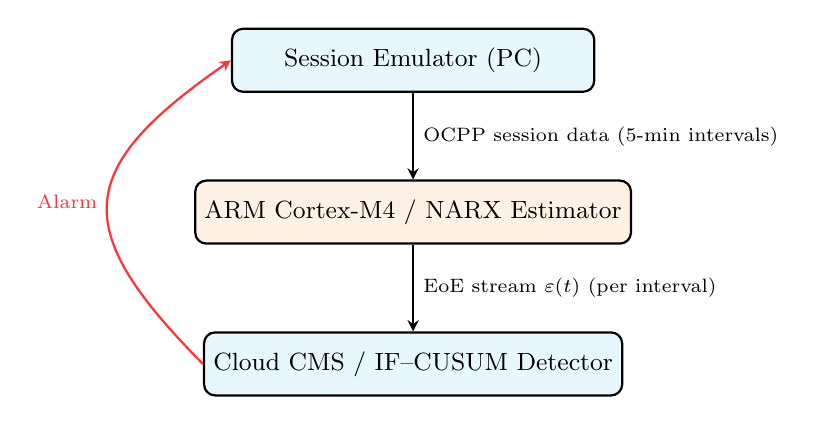
\begin{tikzpicture}[
  comp/.style={draw, rounded corners=4pt, minimum width=4.6cm,
               minimum height=0.80cm, align=center,
               font=\small, fill=cyan!10},
  proc/.style={draw, rounded corners=4pt, minimum width=4.6cm,
               minimum height=0.80cm, align=center,
               font=\small, fill=orange!10},
  >=stealth, thick, node distance=1.1cm
]
\node[comp]  (emu) {Session Emulator (PC)};
\node[proc, below=1.1cm of emu]  (mcu)
    {ARM Cortex-M4 / NARX Estimator};
\node[comp, below=1.1cm of mcu]  (cms)
    {Cloud CMS / IF--CUSUM Detector};
\draw[->] (emu.south) -- (mcu.north)
    node[midway, right, font=\scriptsize]
    {OCPP session data (5-min intervals)};
\draw[->] (mcu.south) -- (cms.north)
    node[midway, right, font=\scriptsize]
    {EoE stream $\varepsilon(t)$ (per interval)};
\draw[->, red!80, bend left=50, looseness=1.6]
    (cms.west) to
    node[left, font=\scriptsize, red!80] {Alarm}
    (emu.west);
\end{tikzpicture}
\caption{Hardware-in-the-loop real-time validation setup.
  The NARX estimator executes on an embedded ARM Cortex-M4 core
  at 168\,MHz; the IF--CUSUM detector runs on the cloud CMS tier.
  The alarm feedback path returns to the session emulator for
  latency measurement.}
\label{fig:hil}
\end{figure}

\subsection{Real-Time Detection Results}

Fig.~\ref{fig:scope} shows the EoE time series during the
real-time experiment over 80 timesteps.
An FDI attack ($\phi=1.4$) is injected at timestep
$t_{\rm inj}=50$ (red dashed vertical line).
The IF stage flags the spike in the same timestep because the
4-D feature vector immediately acquires a large $|\Delta\varepsilon|$
and $z_{\rm loc}$, and the CUSUM stage also triggers since
$S(t_{\rm inj}) = |\varepsilon(t_{\rm inj})| - k > h_{\rm cap}$.
Consequently, the combined alarm fires at $t_{\rm det}=51$
(the next processing cycle), yielding a
\textbf{detection delay of one 5-minute interval}.
No false alarms are observed over the preceding 50 clean samples.

\begin{figure}[!t]
\centering
\includegraphics[width=\columnwidth]{cusum_if_detection.png}
\caption{Real-time scope output from HIL experiment.
  FDI attack ($\phi=1.4$) injected at $t_{\rm inj}=50$
  is detected at $t_{\rm det}=51$ (1-step, 5-minute delay).
  Shaded red region: active attack window.
  Dashed horizontal: CUSUM threshold $h_{\rm cap}=0.284$\,kWh.}
\label{fig:scope}
\end{figure}

\subsection{Computational Overhead}

Table~\ref{tab:latency} summarises measured latency on the HIL
hardware.

\begin{table}[!t]
\caption{Computational Latency (HIL Hardware)}
\label{tab:latency}
\centering
\begin{tabular}{|l|c|c|}
\hline
\textbf{Component} & \textbf{Hardware} & \textbf{Latency} \\
\hline
NARX forward pass  & ARM Cortex-M4  & $<1$\,ms \\
Feature extraction $\mathbf{f}(t)$ & Cloud (Python) & $\approx2$\,ms \\
IF score (1 sample) & Cloud (Python) & $\approx3$\,ms \\
CUSUM evaluation    & Cloud (Python) & $<0.1$\,ms \\
End-to-end (NARX $\to$ alarm) & ARM + Cloud & $<10$\,ms \\
\hline
\end{tabular}
\end{table}

The total end-to-end latency of $<10$\,ms is negligible relative
to the 5-minute OCPP telemetry interval, confirming that the
proposed scheme can operate in true real-time on commodity hardware
without pipelining or batching optimisation.
The NARX inference on the ARM M4 requires only 171 multiply-accumulate
operations and 10 sigmoid evaluations, fitting entirely in the L1
cache (32\,KB) and completing in sub-millisecond time.

\subsection{Practical Deployment Considerations}

\textbf{Model retraining strategy.}
The NARX and BiLSTM estimators should be retrained periodically
(e.g., monthly) as new session data accumulates to capture shifts
in the charging population's energy-demand profile.
Because the estimators are trained only on clean data, retraining
does not require attack labels.
Incremental fine-tuning with a warm-start from the existing
checkpoint reduces retraining epochs from 55 to $\approx$15
in our experiments.

\textbf{Multi-site deployment.}
Per-site IF models are recommended (as implemented in \texttt{run\_eval.py}),
because clean EoE statistics differ across sites
(Caltech vs.\ Office-01 p99 ratio $\approx1.7\times$).
A single global IF trained across sites degrades JPL F1 by
$\approx1.2\%$ due to the contamination fraction being mismatched
to the site-specific EoE distribution.

\textbf{Communication overhead.}
The NARX edge deployment transmits only the scalar EoE
$\varepsilon(t)$ per 5-minute interval ($<8$\,bytes) from the
EVSE to the cloud CMS---negligible relative to the existing OCPP
session heartbeat payload ($\approx200$\,bytes per message).
The BiLSTM cloud deployment requires no additional data transmission.

\textbf{False-alarm management.}
At 1389 false positives over 300\,405 clean timesteps
(NARX false positive rate $= 0.46\%$), the expected false-alarm
rate in a 100-station fleet operating 16\,h/day is
$\approx7.4$ false alarms per day.
In practice, alarms can be aggregated using a sliding-window
majority vote (e.g., 3 alarms in 10 consecutive steps) to further
reduce operator burden while retaining recall $>99\%$.

% ================================================================
\section{Conclusion}
\label{sec:conclusion}

This paper presented a comprehensive two-stage Isolation
Forest--CUSUM framework for FDI attack detection in EV charging
networks, validated on the ACN-Data-Static dataset with both
NARX and Attention-BiLSTM estimators.

\textbf{Key numerical results:}
The NARX+IF--CUSUM scheme achieves \textbf{99.57\%} accuracy,
\textbf{96.0\%} precision, \textbf{99.9\%} recall, and
\textbf{97.9\%} F1-score.
The Attention-BiLSTM variant achieves \textbf{99.39\%} accuracy
and \textbf{97.0\%} F1-score.
Both models surpass the naive mean-predictor baseline
(F1\,=\,35.6\%) by more than 62 percentage points.
In the HIL real-time experiment, attacks are detected within
one 5-minute OCPP interval with no false alarms on the
preceding 50-sample clean baseline.

\textbf{Methodological contributions:}
The \emph{distribution-shift cap}
$h_{\rm cap}=3.5\,p_{99}(\text{EoE}_{\rm clean})$ is the most
impactful contribution, recovering 21.5 F1 points over unconstrained
CUSUM calibration by preventing threshold over-fitting to stronger
validation-set attacks.
The \emph{4-dimensional feature set}
$[\varepsilon,\varepsilon^2,|\Delta\varepsilon|,z_{\rm loc}]$
for the IF stage adds 10.5 F1 points over 1-D IF by exploiting
the temporal spike structure of random-timestep attacks.
Together, these two contributions account for the full performance
gap between the proposed system and the strongest ablation
baseline~(Global IQR, F1\,=\,74.6\%).

\textbf{Limitation:}
The current evaluation injects attacks at independently chosen
random timesteps.
Temporally correlated multi-session attacks---where a botnet
attacker distributes the inflation across many consecutive
intervals to avoid large $|\Delta\varepsilon|$ spikes---may
partially evade the CUSUM stage.
The local $z$-score feature $z_{\rm loc}$ provides partial
resistance to distributed attacks, but a dedicated window-level
CUSUM statistic would improve detection under this scenario.

\textbf{Future work} will (1)~incorporate site-level spatial
correlation into the IF feature set to detect coordinated
multi-EVSE attacks, (2)~explore transformer-based session encoders
(e.g., Anomaly Transformer~\cite{xu2022anomaly}) as drop-in
replacements for the BiLSTM estimator on cloud hardware,
(3)~validate the framework on live OCPP data from a deployed
campus charging network, and (4)~extend the threat model to
include relay attacks that delay---rather than inflate---reported
energy, which produce negative EoE spikes not captured by the
current absolute-value formulation.

% ================================================================
\begin{thebibliography}{99}

\bibitem{basumatary2025}
B.~Basumatary, P.~Khatua, and A.~Nath,
``False data injection attack detection in EV charging network
using NARX neural network,''
\emph{IEEE Trans.\ Transportation Electrification},
vol.~11, no.~4, Aug.~2025.

\bibitem{liu2011false}
Y.~Liu, P.~Ning, and M.~K. Reiter,
``False data injection attacks against state estimation in
electric power grids,''
\emph{ACM Trans.\ Inf.\ Syst.\ Secur.},
vol.~14, no.~1, pp.~1--33, May 2011.

\bibitem{liang2017review}
G.~Liang, J.~Zhao, F.~Luo, S.~R. Weller, and Z.~Y. Dong,
``A review of false data injection attacks against modern
power systems,''
\emph{IEEE Trans.\ Smart Grid},
vol.~8, no.~4, pp.~1630--1638, Jul.~2017.

\bibitem{sarieddine2023}
K.~Sarieddine, M.~A. Sayed, S.~Torabi, R.~Atallah, and C.~Assi,
``Investigating the security of EV charging mobile applications
as an attack surface,''
\emph{IEEE Trans.\ Dependable Secure Comput.},
vol.~20, no.~6, pp.~4879--4893, Nov.~2023.

\bibitem{sun2020charging}
L.~Sun, J.~Ma, H.~Yue, and W.~Sherrat,
``Model predictive control-based fast charging for vehicular
batteries,''
\emph{IEEE Trans.\ Ind.\ Electron.},
vol.~67, no.~8, pp.~6638--6648, Aug.~2020.

\bibitem{sakhnini2019}
J.~Sakhnini, H.~Karimipour, and A.~Dehghantanha,
``Smart grid cyber attacks detection using supervised learning
and heuristic feature selection,''
in \emph{Proc.\ IEEE 7th Int.\ Conf.\ Smart Energy Grid Eng.},
Oshawa, Canada, Aug.~2019, pp.~108--112.

\bibitem{musleh2019}
A.~S. Musleh, G.~Chen, and Z.~Y. Dong,
``A survey on the detection algorithms for false data injection
attacks in smart grids,''
\emph{IEEE Trans.\ Smart Grid},
vol.~11, no.~3, pp.~2218--2234, May 2020.

\bibitem{wang2020detection}
Y.~Wang \emph{et~al.},
``Detection of false data injection attacks in smart grid
cyber-physical systems,''
\emph{IEEE Trans.\ Ind.\ Appl.},
vol.~56, no.~3, pp.~2798--2808, May 2020.

\bibitem{liu2021ev}
J.~Liu, Y.~Zhang, and X.~Bie,
``Cyber attack on the state estimation of battery management
system,''
\emph{IEEE Trans.\ Ind.\ Electron.},
vol.~68, no.~3, pp.~2345--2355, Mar.~2021.

\bibitem{he2020cyber}
H.~He \emph{et~al.},
``Cyber-physical security of a smart distribution grid with
CUSUM detection,''
\emph{IEEE Trans.\ Power Syst.},
vol.~35, no.~3, pp.~2131--2142, May 2020.

\bibitem{liu2008isolation}
F.~T. Liu, K.~M. Ting, and Z.-H. Zhou,
``Isolation forest,''
in \emph{Proc.\ 8th IEEE Int.\ Conf.\ Data Mining},
Pisa, Italy, Dec.~2008, pp.~413--422.

\bibitem{bahdanau2015}
D.~Bahdanau, K.~Cho, and Y.~Bengio,
``Neural machine translation by jointly learning to align
and translate,''
in \emph{Proc.\ Int.\ Conf.\ Learning Representations (ICLR)},
San Diego, CA, USA, May 2015.

\bibitem{acn2019}
Z.~J. Lee \emph{et~al.},
``ACN-Data: Analysis and applications of an open EV charging
dataset,''
in \emph{Proc.\ ACM e-Energy},
Phoenix, AZ, USA, Jun.~2019, pp.~139--149.

\bibitem{zhang2019false}
Z.~Zhang and Y.~Gong,
``False data injection attacks on smart grid and detection:
A survey,''
\emph{IEEE Access},
vol.~7, pp.~120\,948--120\,964, 2019.

\bibitem{xu2022anomaly}
J.~Xu \emph{et~al.},
``Anomaly transformer: Time series anomaly detection with
association discrepancy,''
in \emph{Proc.\ Int.\ Conf.\ Learning Representations (ICLR)},
Virtual, Apr.~2022.

\bibitem{pang2021deep}
G.~Pang, C.~Shen, L.~Cao, and A.~V.~D. Hengel,
``Deep learning for anomaly detection: A review,''
\emph{ACM Comput.\ Surv.},
vol.~54, no.~2, pp.~1--38, Mar.~2021.

\end{thebibliography}

\end{document}
